%&tex
% !BIB TS-program = bibtex
% !TeX encoding = UTF-8
% !TeX spellcheck = de_DE
% !TeX root = Presentation.tex

\documentclass[10pt]{beamer}

\usepackage[utf8]{inputenc}
\usepackage[ngerman]{babel}

\usetheme{metropolis}
\usepackage{appendixnumberbeamer}

\usepackage{booktabs}
\usepackage[scale=2]{ccicons}

\usepackage{verbatim}

\usepackage{ctable}
\usepackage{float}
\usepackage{multirow}
\usepackage{adjustbox}

\usepackage{xcolor}
\usepackage{colortbl}

\usepackage{textcomp}

\newcommand{\themename}{\textbf{\textsc{metropolis}}\xspace}

\title{API-Usability}
\subtitle{Effekte der Konstruktoren}
\date{21. August 2018}
\author{Elias Hofele, David Oberacker und Calvin Urankar}
\institute{Institut für Telematik, Telecooperation Office (TECO), Karlsruher Institut für Technologie}
\titlegraphic{\hfill
\includegraphics[height=0.5cm]{TECO_Logo.jpg}}

\begin{document}
    
    \maketitle
    
%    \begin{frame}{Table of contents}
%    \setbeamertemplate{section in toc}[sections numbered]
%    \tableofcontents[hideallsubsections]
%	\end{frame}

\section{Motivation}

	\begin{frame}[fragile]{APIs \& Benutzbarkeit}
		\metroset{block=fill}
		\begin{block}{Usability}
			\textit{Extent to which a system, product or service can be used by specified users to achieve specified goals with effectiveness,
				efficiency and satisfaction in a specified context of use.}	
			\hfill - ISO 9241-11
		\end{block}
		\vspace{\baselineskip}
		\begin{block}{API-Usability}
			\textit{[...] four main research questions, which characterize fundamental aspects of usability: understandability, abstraction level, reusability, and learnability.}	
			\hfill - Piccioni, Furia \& Meyer~\cite{6681333}
		\end{block}
%		\begin{block}{API Usability}
%			\textit{The first-level arributes are: Knowability, Operability, Efficiency, Robustness, Safety, Subjective satisfaction.}	
%			\hfill - Mosqueira-Rey, et. al
%		\end{block}
	
	\end{frame}

	\begin{frame}[fragile]{Default vs. Required}
		\begin{columns}[T,onlytextwidth]
			
			\begin{column}{0.45\textwidth}
				\begin{center}\textit{create-set-call}\end{center}
				\begin{verbatim}
					var foo = new FooClass();
					foo.setBar(barValue);
					foo.use();
				\end{verbatim}
			\end{column}
			\vrule{}
			\begin{column}{0.02\textwidth}
			\end{column}
			\begin{column}{0.53\textwidth}
				\begin{center}\textit{create-call}\end{center}
				\begin{verbatim}
					var foo = new FooClass(barValue);
					foo.use();
				\end{verbatim}
			\end{column}
			
		\end{columns}
	\end{frame}

	\begin{frame}{Verwandte Arbeiten}
		\begin{quote}
			We found the create-set-call pattern to be more
			usable than, and preferred to, required constructors.
		\end{quote}
		\hfill - Stylos \& Clarke~\cite{Stylos:2007:UIR:1248820.1248828}\\
		\vspace{\baselineskip}
		\vspace{\baselineskip}
		\begin{quote}
			In our study, however, the participants had no particular
			difficulties with using constructors with arguments [...]. 
		\end{quote}
		\hfill - Piccioni, Furia \& Meyer~\cite{6681333}
	
	
	\end{frame}

\section{Forschungsfrage \& Hypothese}

	\begin{frame}[standout]{Hypothese}
		Semantische Fehler im Quellcode werden mit Default-Konstruktoren schneller entdeckt
		\begin{center}\small{und}\end{center}
		Konstruktoren haben keinen Einfluss auf das Finden von syntaktischen Fehlern.
	\end{frame}

	\begin{frame}{Nutzerstudie}
		\begin{itemize}
			\item Quantitativer Ansatz
			\begin{itemize}
				\item Web-basierte Studie\\
				\item Within subjects\\
			\end{itemize}
			\vspace{\baselineskip}
			\item Fehlersuche\\
			\vspace{\baselineskip}
			\item Vier Quellcode-Ausschnitte pro Proband\\
		\end{itemize}
	\end{frame}

	\begin{frame}{Variablen}
		\begin{columns}[T,onlytextwidth]
	
			\column{0.5\textwidth}
			Unabhängige Variablen
			\begin{itemize}
				\item Art des Konstruktors:
				\begin{itemize}
					\item Default
					\item Required
				\end{itemize}
				\item Art des Fehlers:
				\begin{itemize}
					\item Syntaktisch
					\item Semantisch
				\end{itemize}
			\end{itemize}			
		
			\column{0.5\textwidth}
			Abhängige Variablen
			\begin{itemize}
				\item Anzahl gefundener Fehler
				\item Zeit
				\item Lesefokus (Areas of Interest)
				\begin{itemize}
					\item Dokumentation
					\item Pre-Defekt
					\item Defekt
					\item Post-Defekt
				\end{itemize}
			\end{itemize}
			
		\end{columns}	
	\end{frame}

\section{Experimentalaufbau}

	\begin{frame}{Aufgabenanforderungen}
		\begin{itemize}
			\item Plausibilität\\
				\begin{itemize}
					\item Nutzung der Standard-Java-API
				\end{itemize}
			\vspace{\baselineskip}
			\item Komplexität\\
			\vspace{\baselineskip}
			\item Untereinander unabhängig\\
            \vspace{\baselineskip}
			\item Länge
			\begin{itemize}
				\item $\sim$ 100 Zeilen Dokumentation
				\item $\sim$ 80 Zeilen Code
			\end{itemize}
		\end{itemize}
	\end{frame}

	\begin{frame}{Peter  i}
		\begin{figure}
			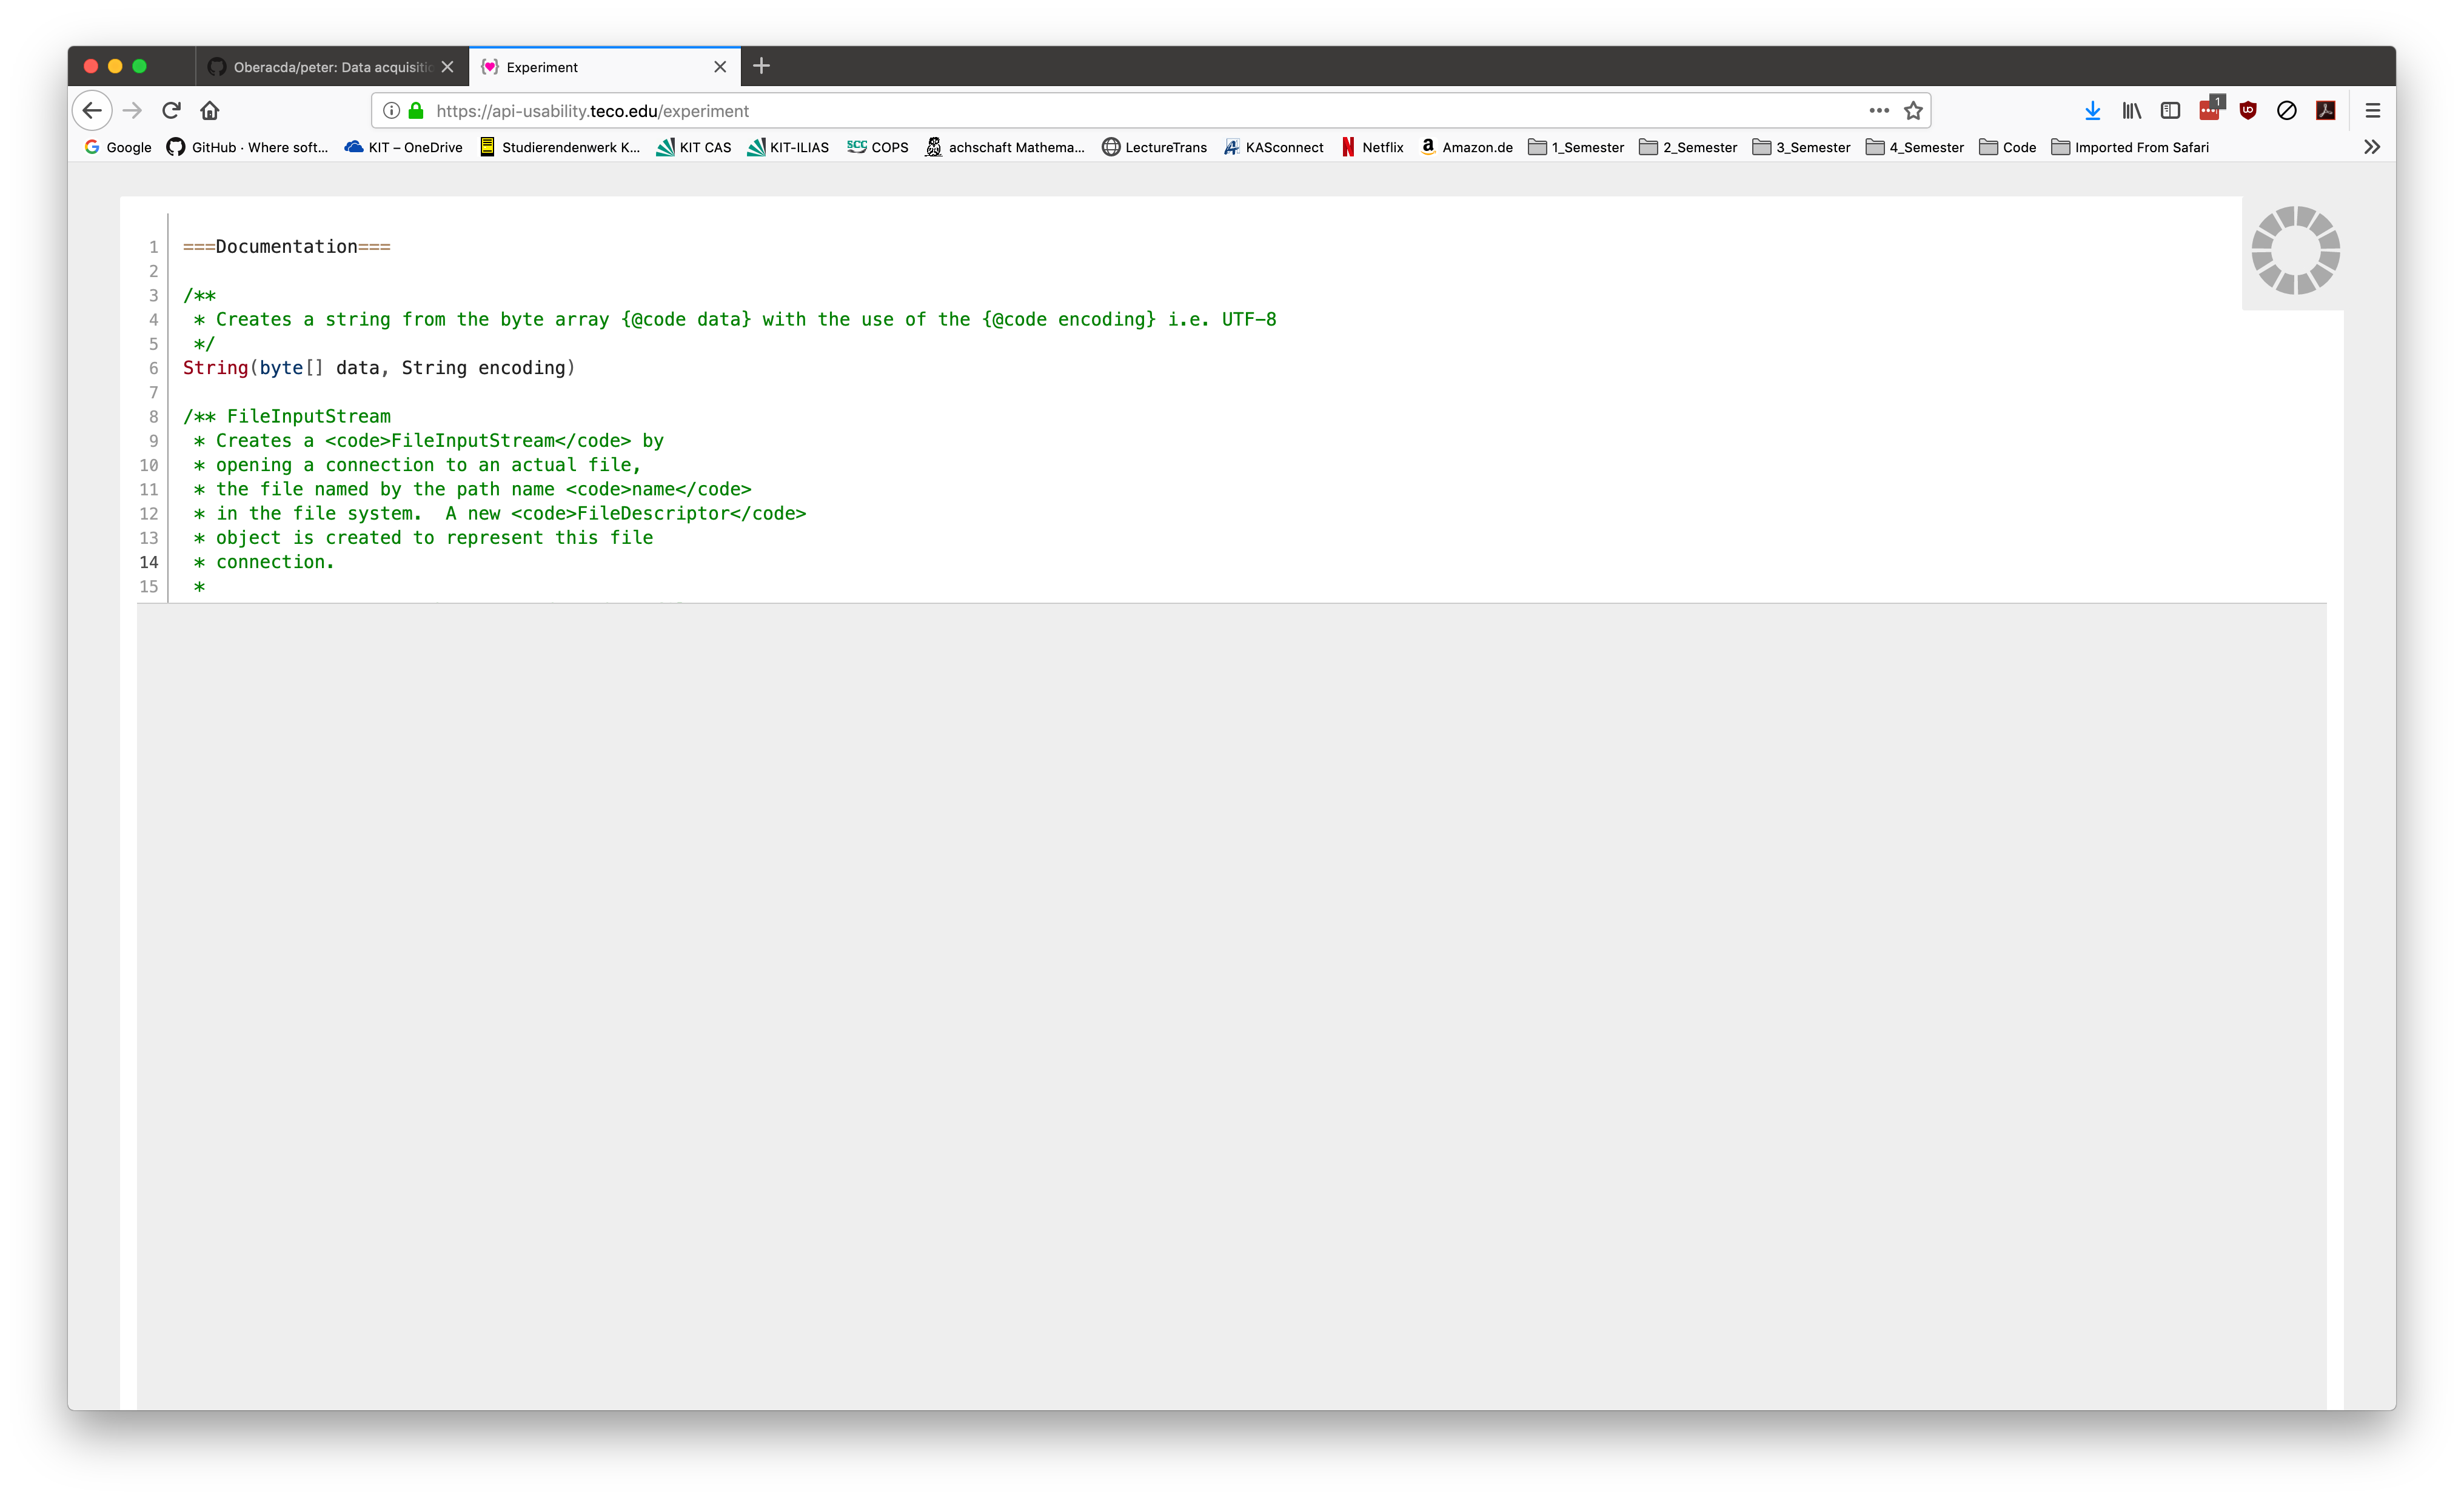
\includegraphics[scale=0.15]{graphics/peter_window.png}
			\caption{\label{fig:peter_window.png} Probanden sahen stets nur einen Ausschnitt des Quellcodes, welchen sie jedoch nach oben und unten bewegen konnten.}
		\end{figure}
	\end{frame}

	\begin{frame}{Peter  ii}	
		\begin{figure}
			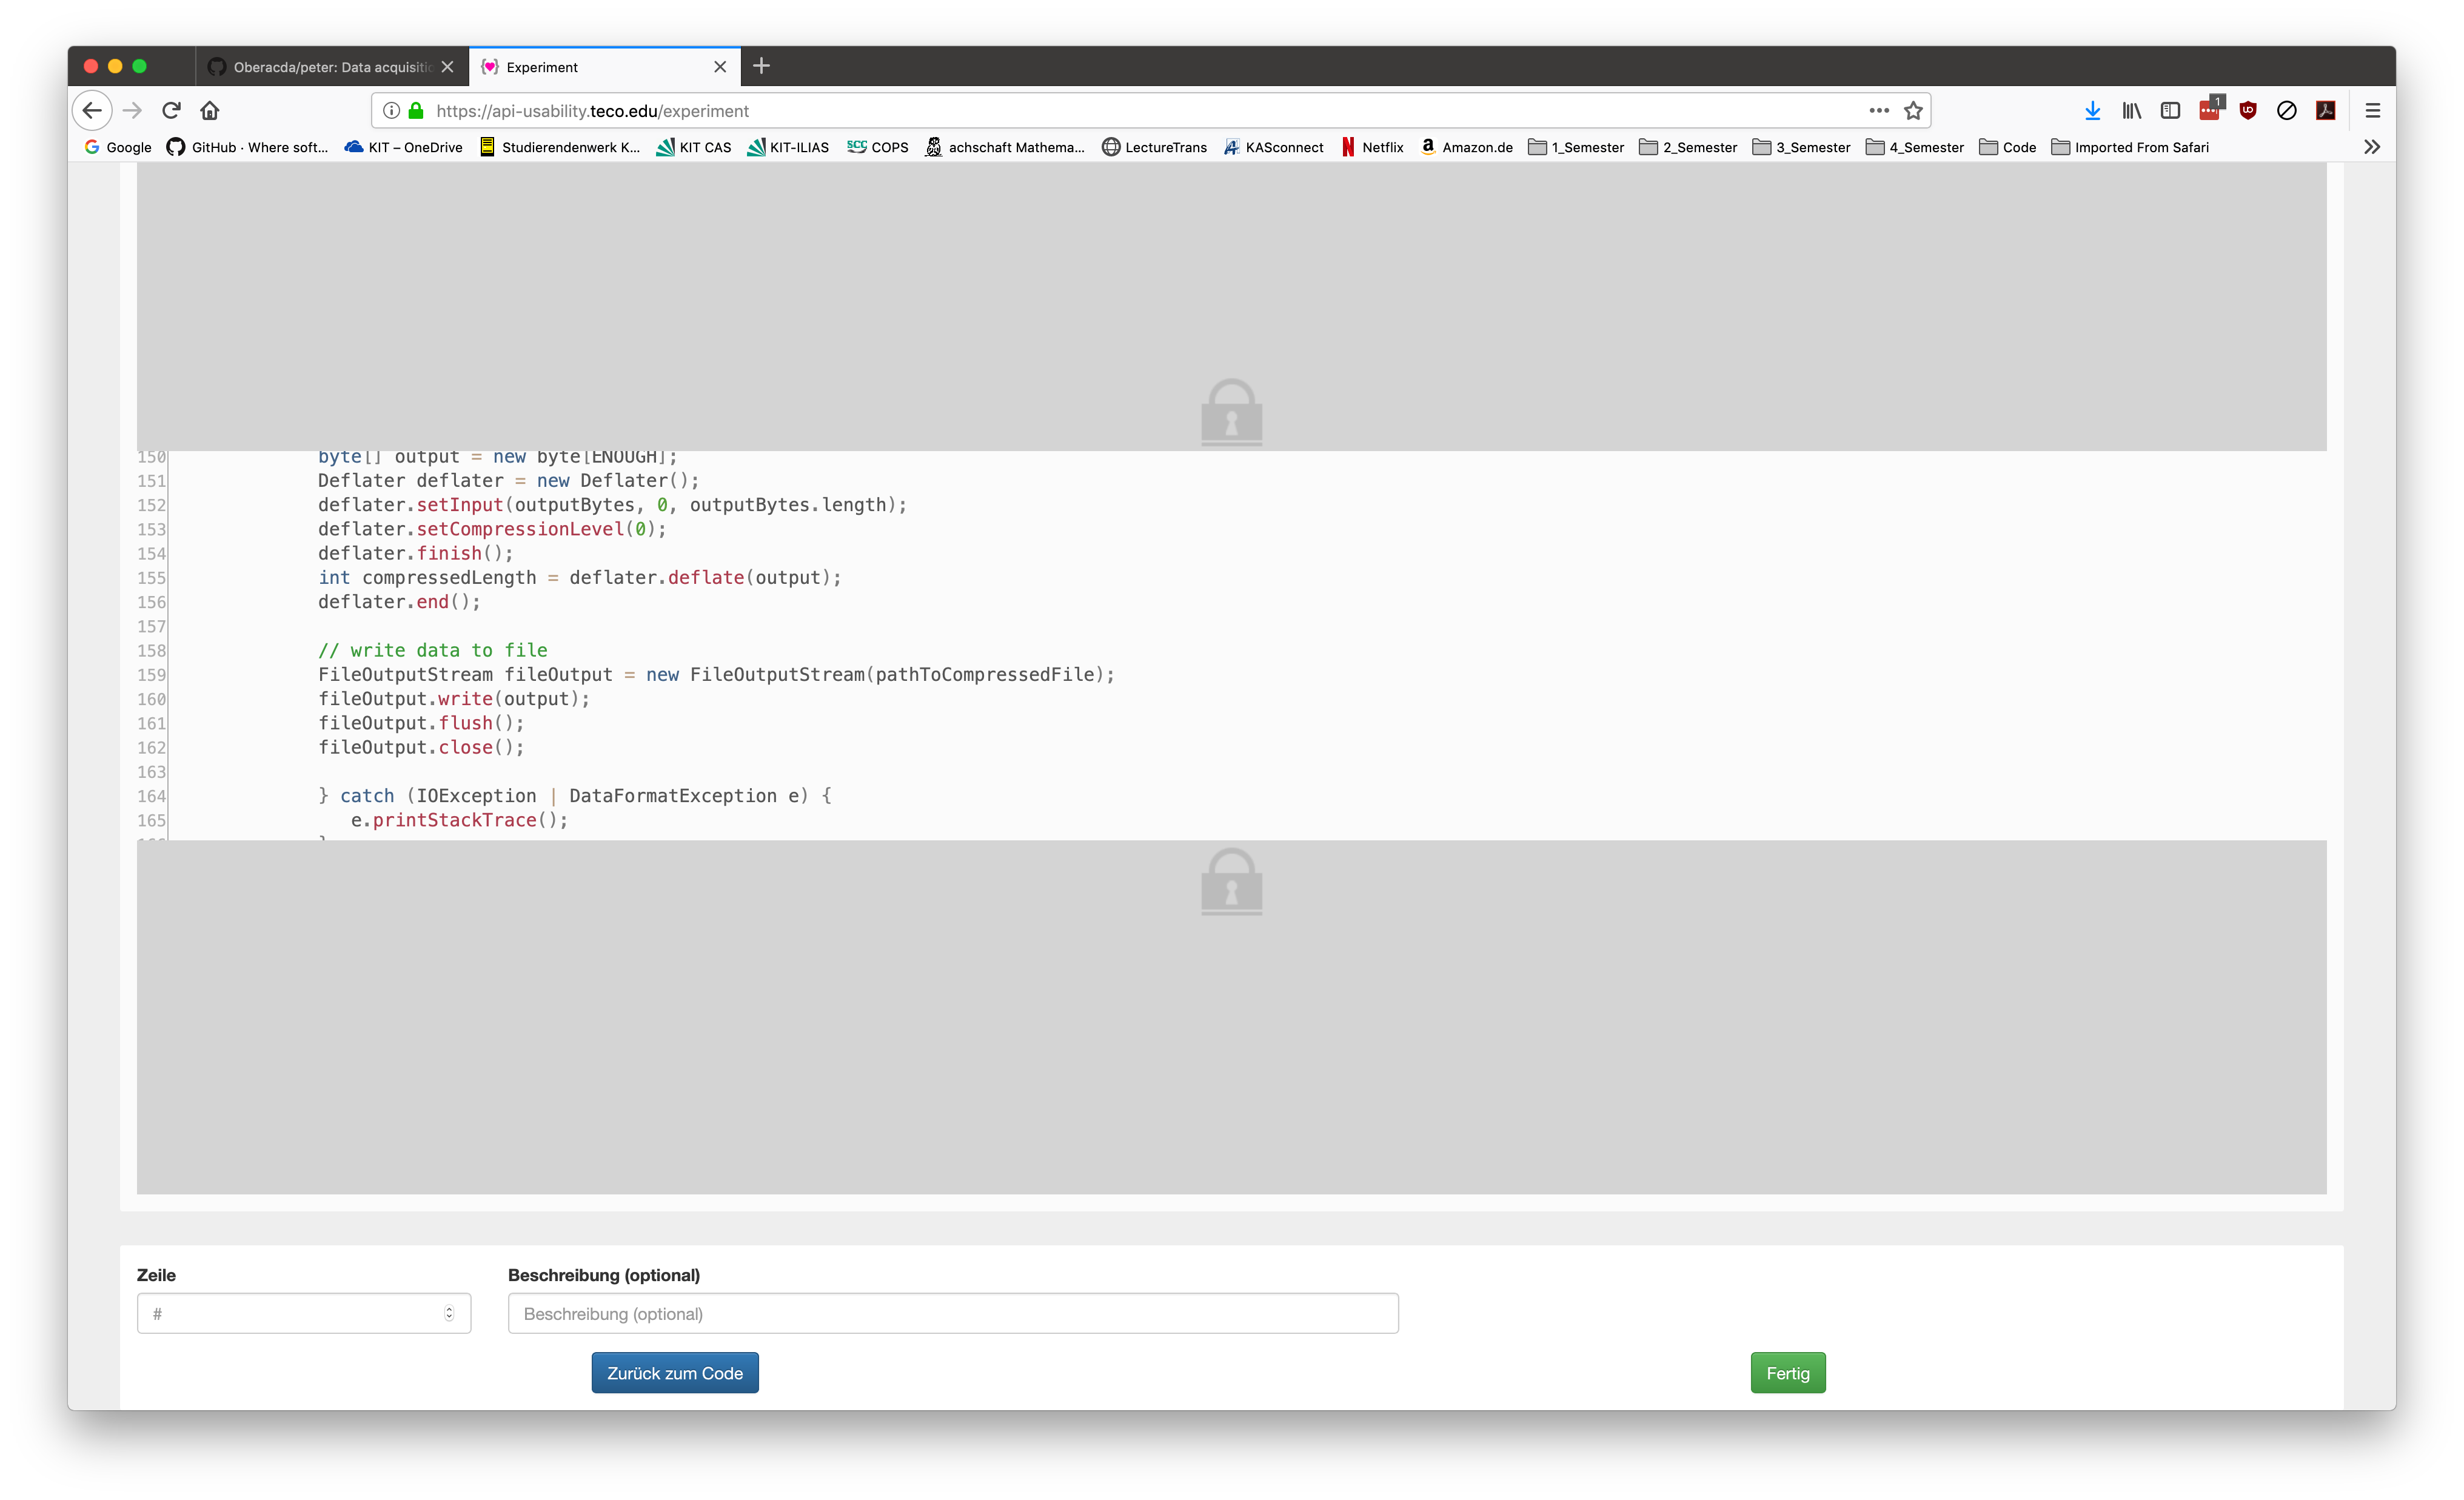
\includegraphics[scale=0.15]{graphics/peter_correction.png}
			\caption{\label{fig:peter_correction.png} Durch das Drücken der Leertaste konnten Probanden indizieren das sie den Fehler gefunden hatten.}
		\end{figure}
	\end{frame}

\section{Resultate}

	\begin{frame}{Stichprobenbeschreibung}
    
    \begin{itemize}
        \item 31 Probanden für semantischen Aufgaben
        \item 28 Probanden für syntaktische Aufgaben
        \item Geschlecht
        \begin{itemize}
            \item 20 Männer
            \item 3 Frauen
            \item 8 ohne Angabe
        \end{itemize}
        \item Alter zwischen 16 - 27 ($\tilde{x} = 22$ Jahre)
        \item 6 Jahre Programmiererfahrung (Median)
        
    \end{itemize}
	 
	\end{frame}

	\begin{frame}{Bearbeitungszeit nach Konstruktor}
		\begin{figure}
			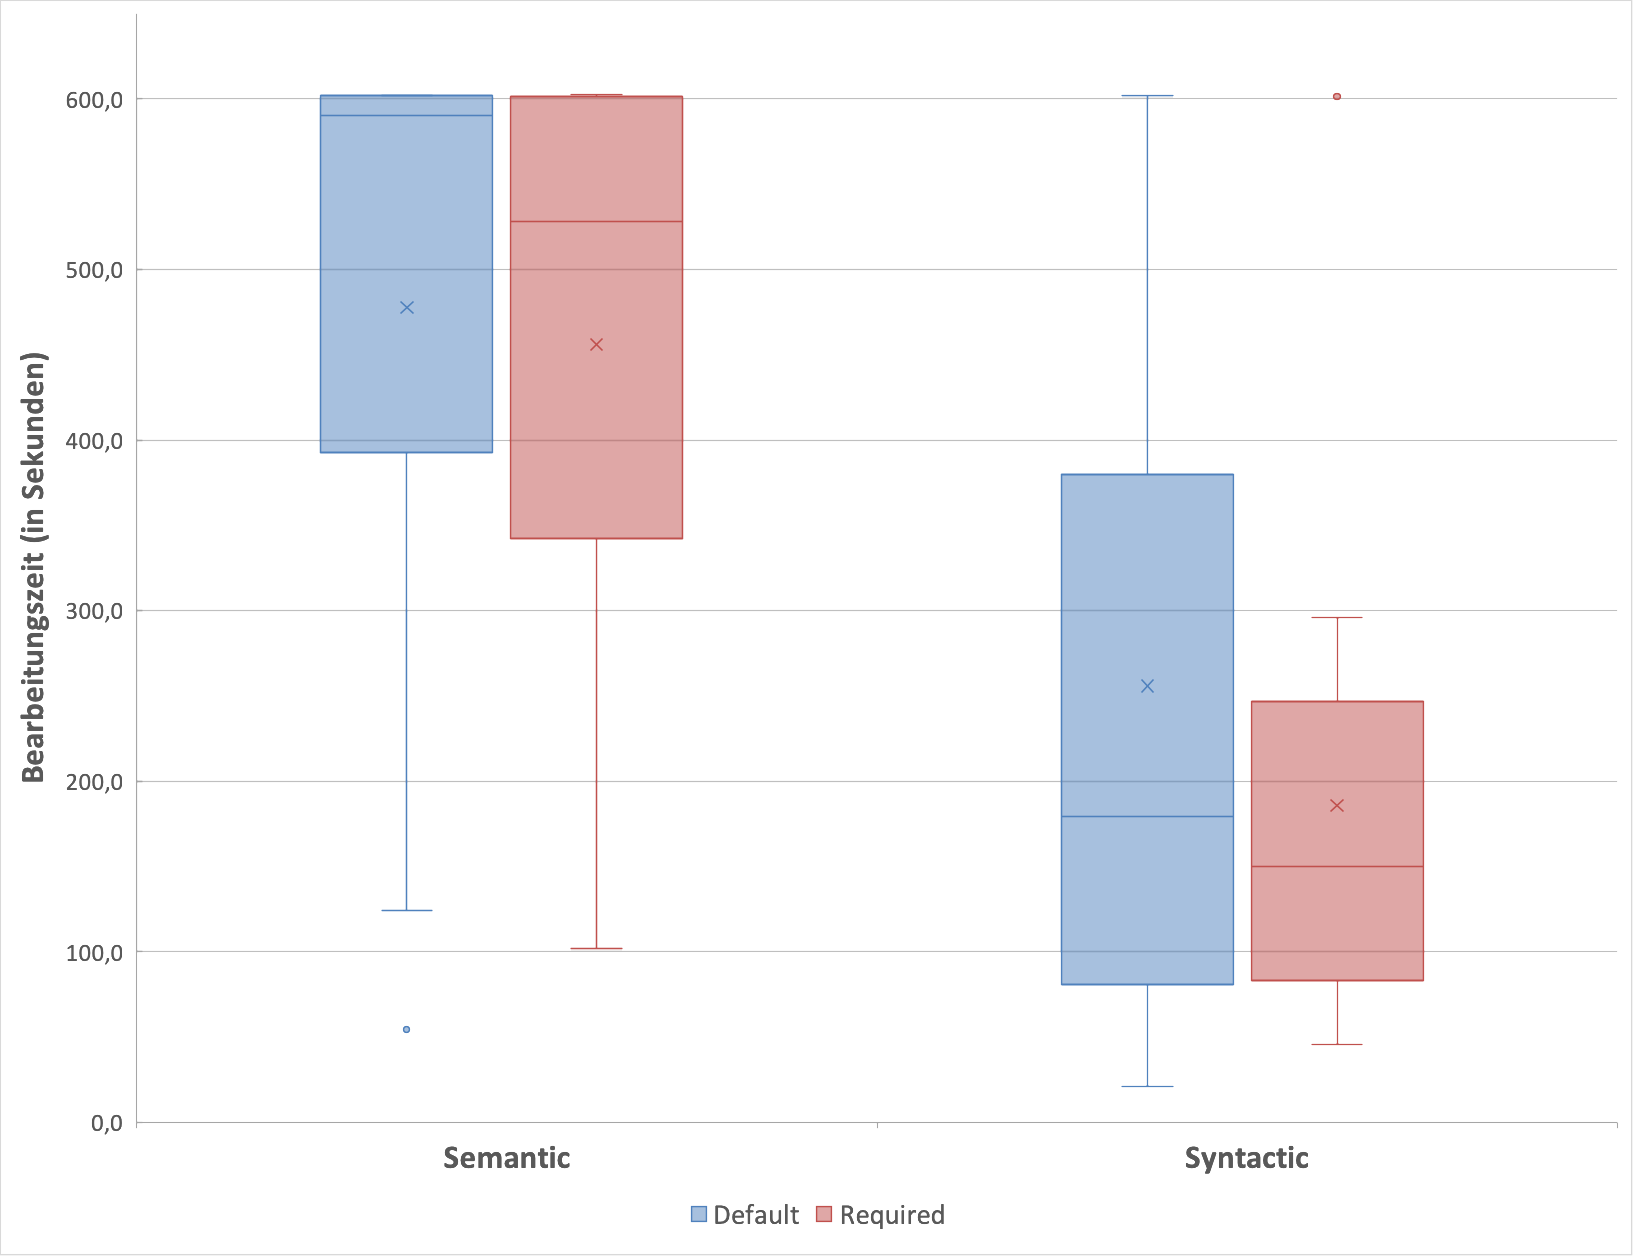
\includegraphics[scale=0.32]{graphics/box_time-constructor.png}
			\caption{\label{fig:box_time-constructor.png} Die Bearbeitungszeit nach Art des Konstruktors}
		\end{figure}
	\end{frame}

	\begin{frame}{Erfolgsquote nach Konstruktor}
		\begin{figure}
			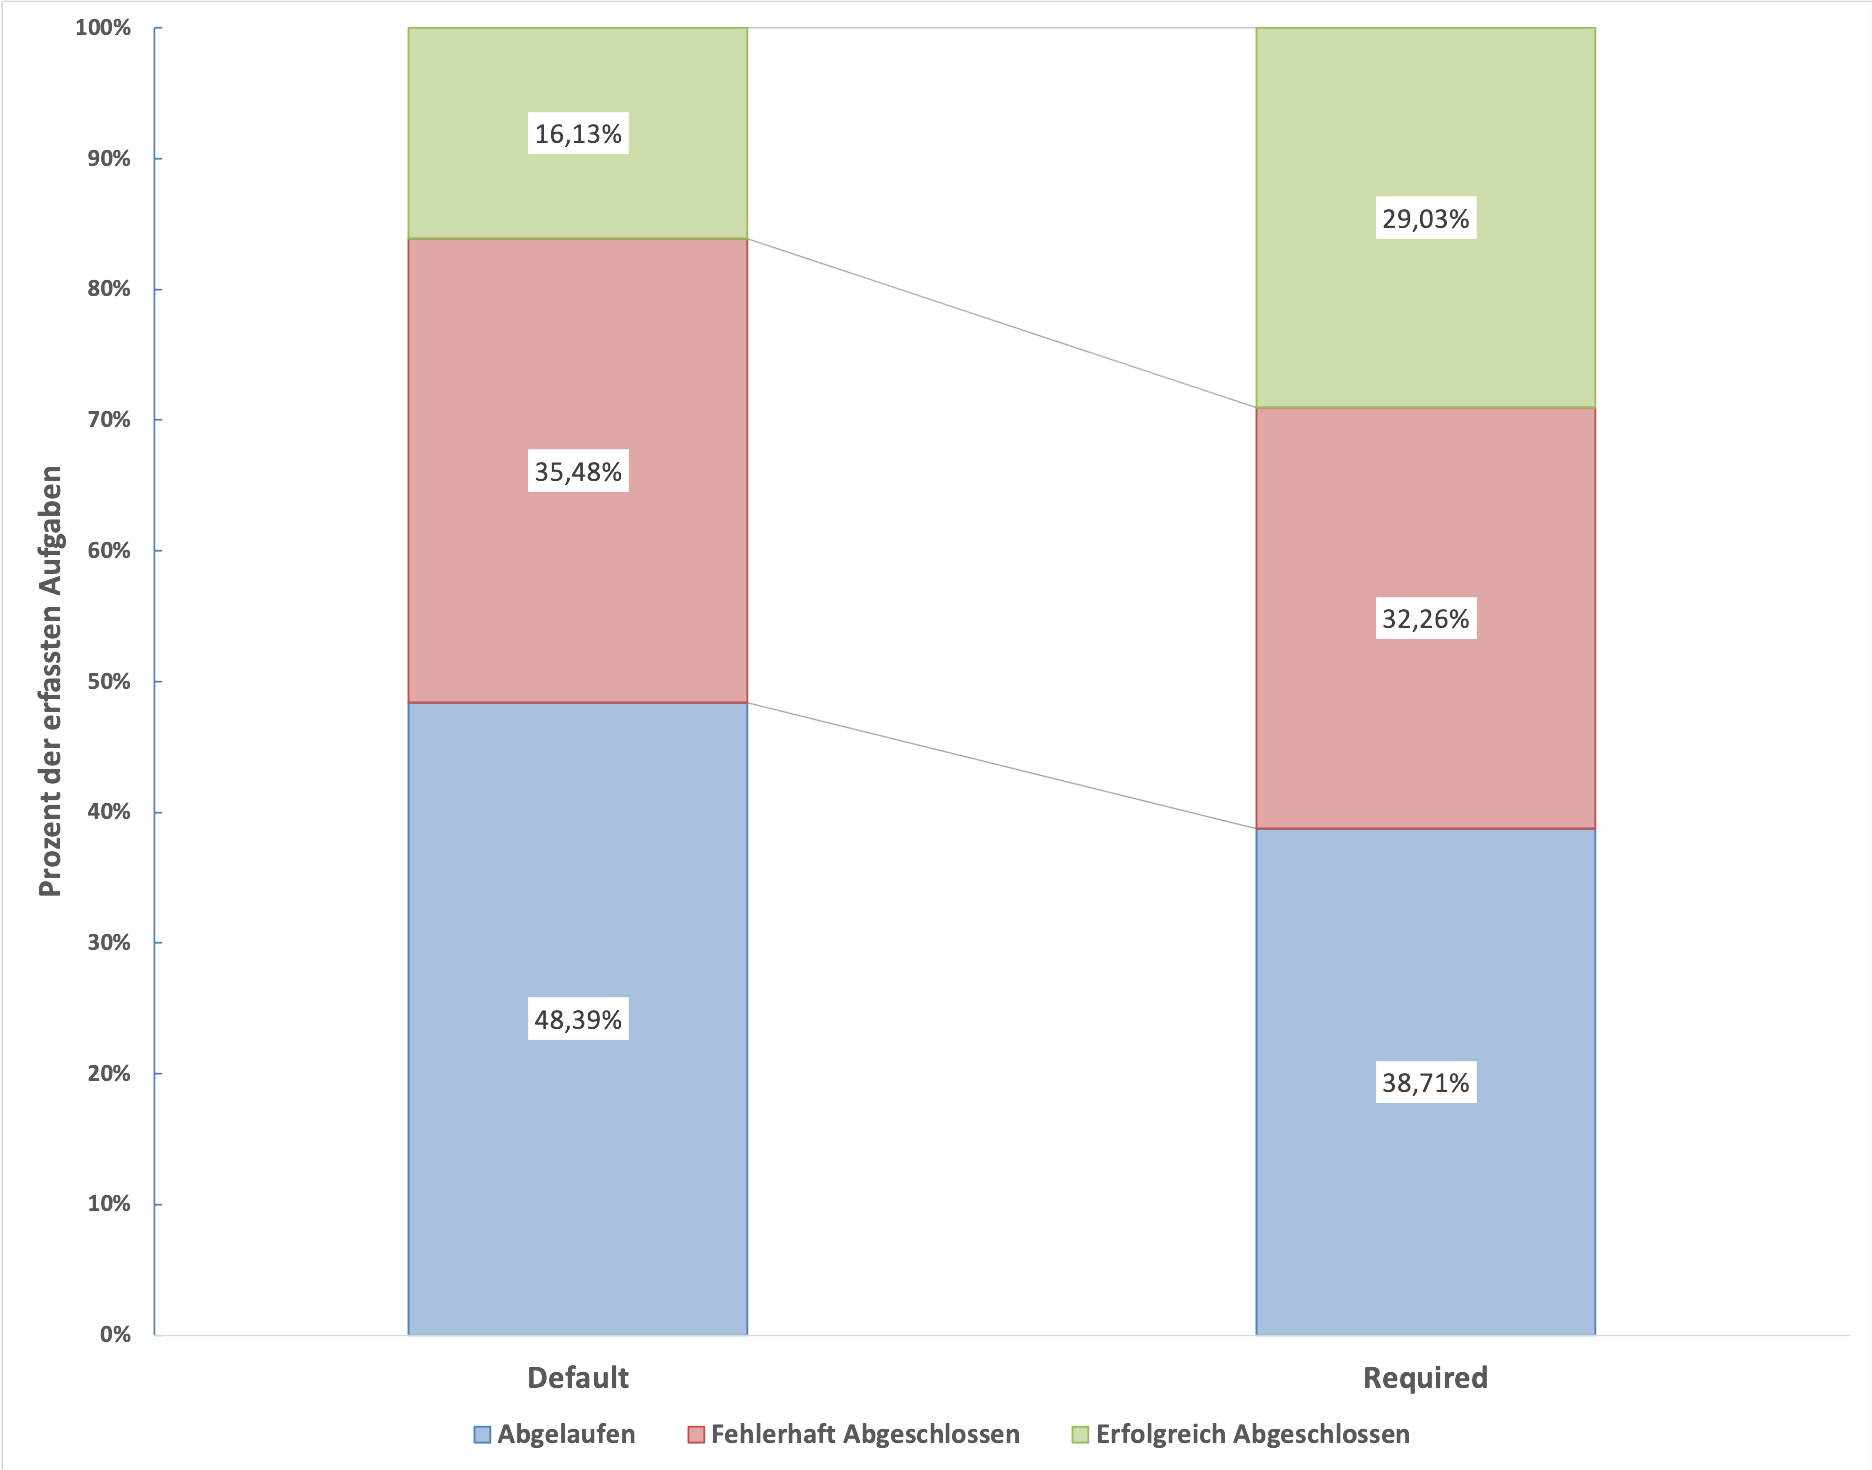
\includegraphics[width=0.76\textwidth]{graphics/bar_result_sem.png}
			\caption{\label{fig:bar_result_sem.png} Resultat der semantischen Aufgaben nach Art des Konstruktors}
		\end{figure}
	\end{frame}

	\begin{frame}{Validität}
		\begin{columns}[T,onlytextwidth]
	
			\column{0.5\textwidth}
			Intern
			\begin{itemize}
				\item Verständlichkeit der Konstruktoren abhängig vom Verständnis des allgemeinen Problems/Sachgebiets
				\item Web-basiert (keine volle Kontrolle über das Verhalten der Teilnehmer)
			\end{itemize}
		
			\column{0.5\textwidth}
			Extern
			\begin{itemize}
				\item Ungewohnte Umgebung (Peter)
				\item Nicht repräsentativ für größere, komplexere APIs
				\item default-Konstruktoren nicht immer sinnvoll
				\item Nur ein Aufgabentyp: Fehlersuche
				\item Studie $\neq$ reale Bedingungen
			\end{itemize}
		\end{columns}	
	
	\end{frame}
	
	\begin{frame}[standout]{Fazit}
		Unsere Hypothese wird durch die Resultate \underline{nicht} bestätigt.
	\end{frame}

\section{Vielen Dank für eure Aufmerksamkeit}

\appendix

	\begin{frame}[standout]
		Fragen?
	\end{frame}

	\begin{frame}[allowframebreaks]{Bibliographie}
		\bibliography{Presentation}
		\bibliographystyle{abbrv}
	\end{frame}

	\begin{frame}{Bearbeitungszeit nach AOI (semantic)}
		\begin{figure}
			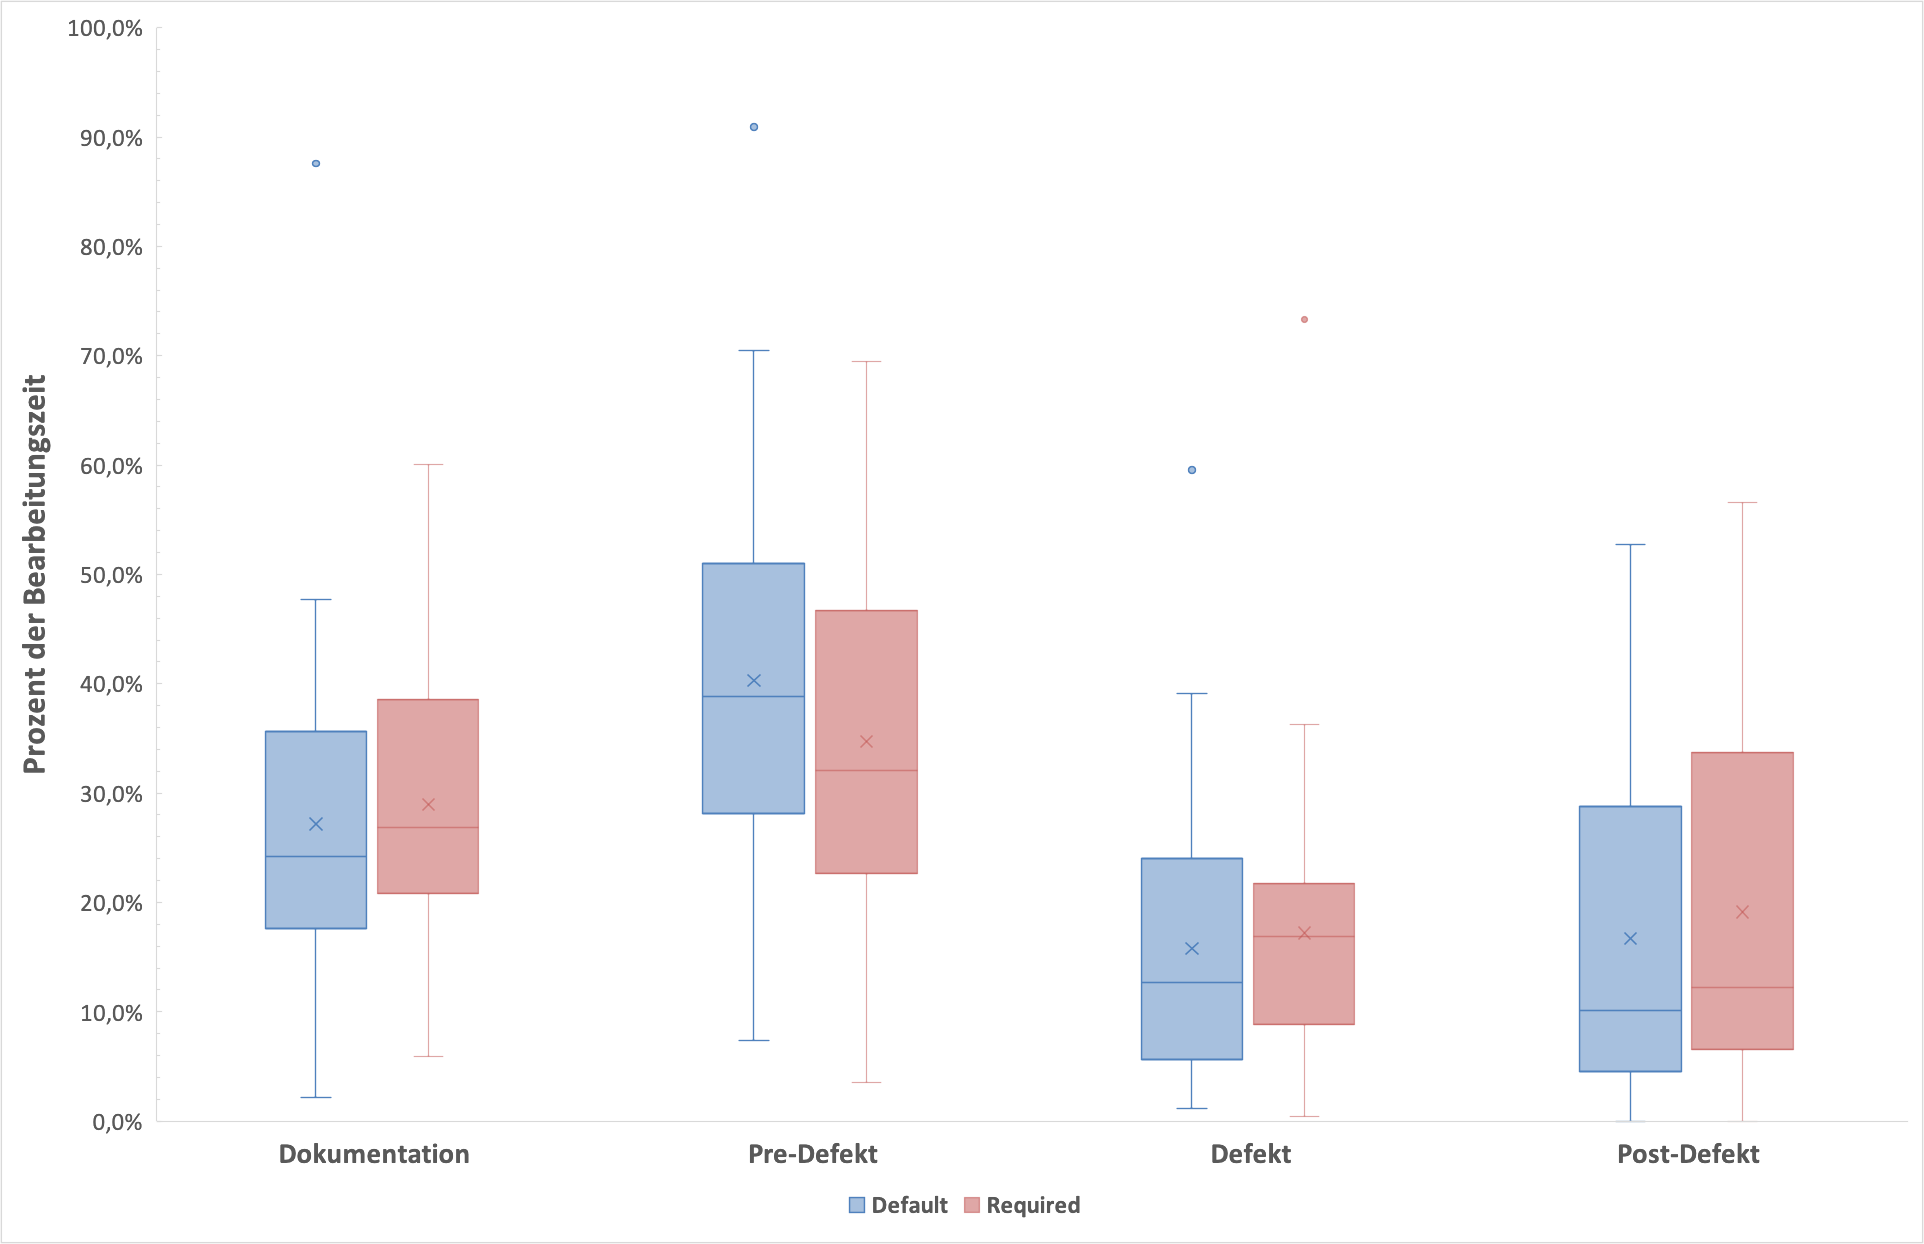
\includegraphics[width=0.8\textwidth]{graphics/box_time-aoi_sem.png}
			\caption{
				\label{fig:box_time-aoi_sem.png} 
				Die Bearbeitungszeit der verschiedenen Areas of Interest (AOI) der semantischen Aufgaben nach Art des Konstruktors.
			}
		\end{figure}
	\end{frame}

	\begin{frame}{Bearbeitungszeit nach AOI (syntactic)}
		\begin{figure}
			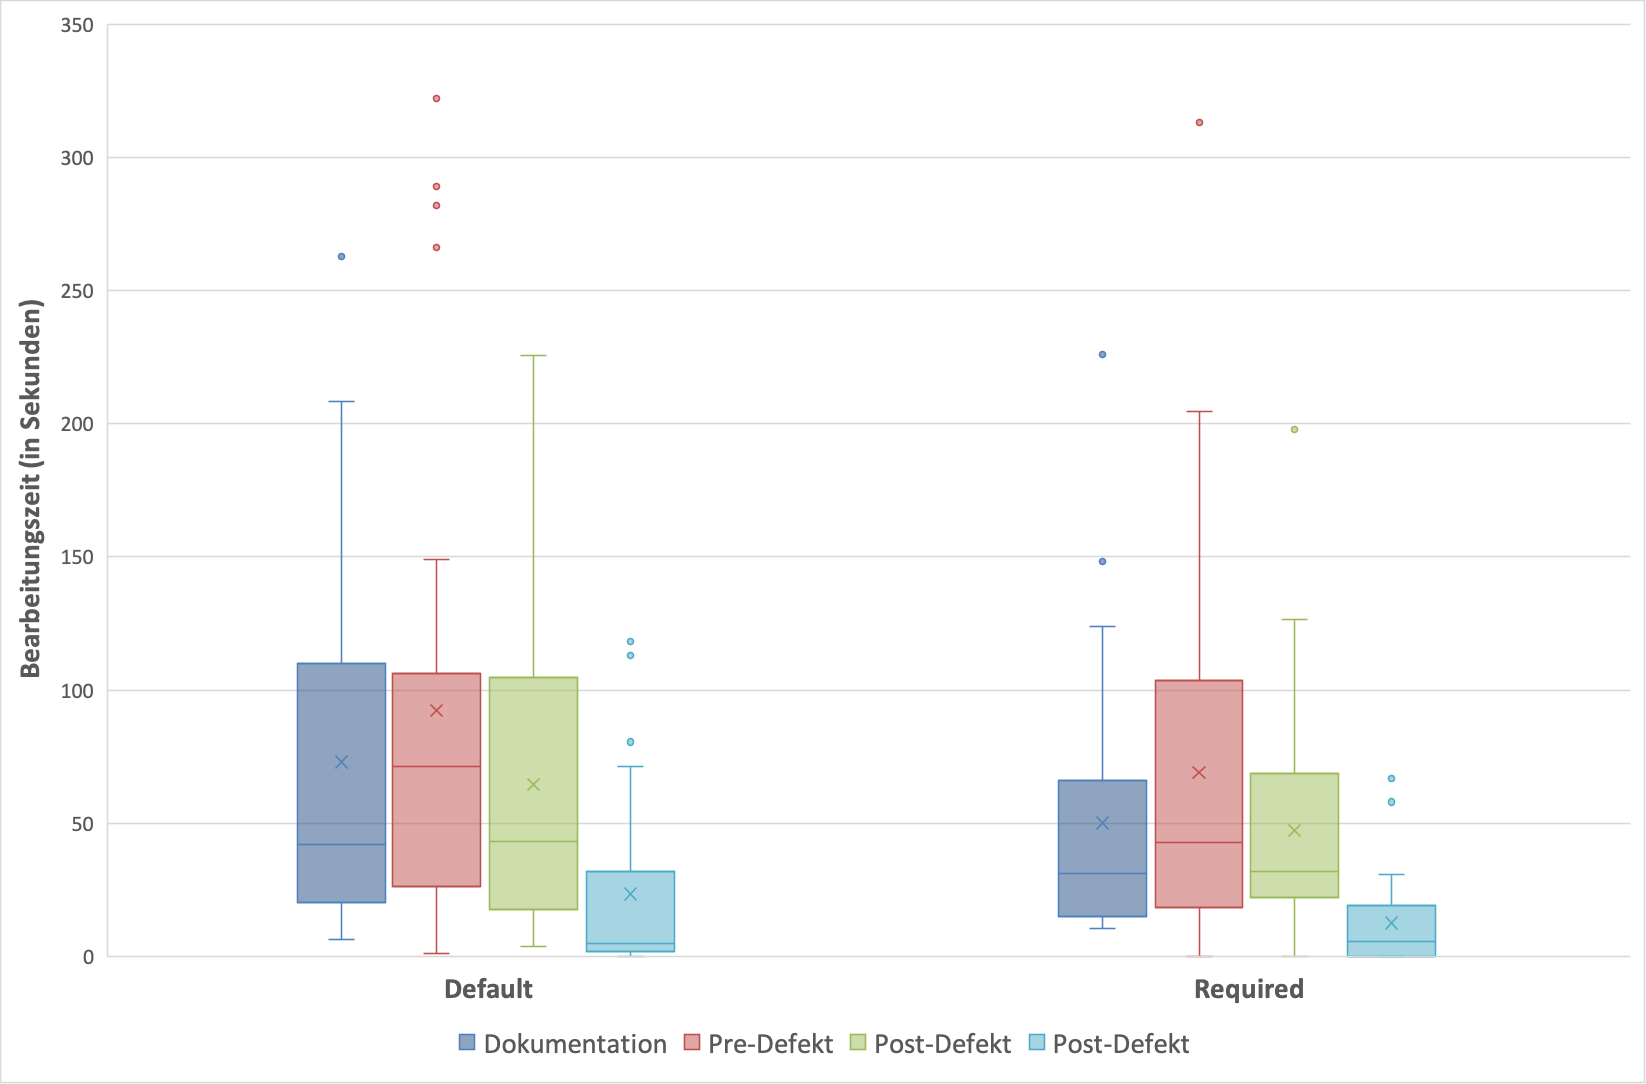
\includegraphics[width=0.8\textwidth]{graphics/box_time-aoi_syn.png}
			\caption{
				\label{fig:box_time-aoi_syn.png} 
				Die Bearbeitungszeit der verschiedenen Areas of Interest (AOI) der syntaktischen Aufgaben nach Art des Konstruktors.
			}
		\end{figure}
	\end{frame}

	\begin{frame}{Erfahrung der Probanden}
		\begin{figure}
			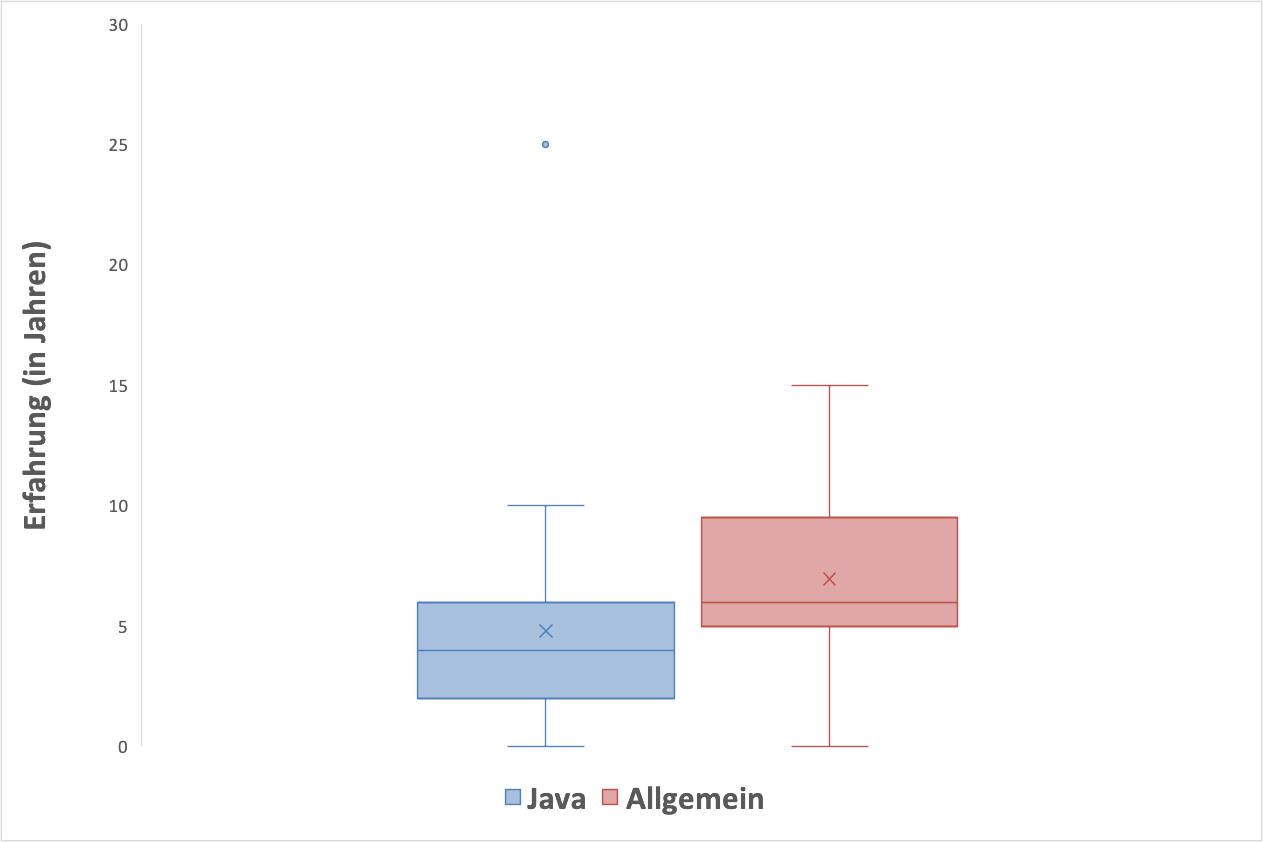
\includegraphics[width=0.85\textwidth]{graphics/box_experience_years.png}
			\caption{
				\label{fig:box_experience_years.png} 
			Programmiererfahrung der Probanden in Jahren
			}
		\end{figure}
	\end{frame}

	\begin{frame}{Deskriptive Statistik}
		\centering
		\adjustbox{max height=\dimexpr\textheight-5.0cm\relax, max width=\textwidth}{
			\begin{tabular}{c p{7.335em} r r r r r r}
				\multicolumn{2}{c}{\multirow{2}[0]{*}{\textcolor[rgb]{ .086,  .212,  .361}{}}} & 
				\multicolumn{1}{c}{\multirow{2}[0]{*}{\textcolor[rgb]{ .086,  .212,  .361}{N}}} & 
				\multicolumn{1}{c}{\multirow{2}[0]{*}{\textcolor[rgb]{ .086,  .212,  .361}{Mean}}} &
				\multicolumn{1}{c}{\multirow{2}[0]{*}{\textcolor[rgb]{ .086,  .212,  .361}{Median}}} & 
				\multicolumn{1}{c}{\multirow{2}[0]{*}{\textcolor[rgb]{ .086,  .212,  .361}{Std. Deviation}}} & 
				\multicolumn{2}{c}{\textcolor[rgb]{ .086,  .212,  .361}{Percentiles}} \\
				
				\multicolumn{2}{c}{} &
				\multicolumn{1}{c}{} &
				\multicolumn{1}{c}{} &
				\multicolumn{1}{c}{} & 
				\multicolumn{1}{c}{} &
				\multicolumn{1}{c}{\multirow{2}[0]{*}{\textcolor[rgb]{ .086,  .212,  .361}{25}}} &
				\multicolumn{1}{c}{\multirow{2}[0]{*}{\textcolor[rgb]{ .086,  .212,  .361}{75}}} \\
				
				\multicolumn{6}{l}{\textcolor[rgb]{ .086,  .212,  .361}{Semantische Aufgabe}} & \multicolumn{2}{c}{\textcolor[rgb]{ .149,  .29,  .376}{}} \\
				
				\toprule
				
				\multicolumn{1}{c}{\cellcolor[rgb]{ .851,  .851,  .851}} &
				\textcolor[rgb]{ .086,  .212,  .361}{\cellcolor[rgb]{ .851,  .851,  .851}Default} & 
				\cellcolor[rgb]{ 1,  1,  1}\textcolor[rgb]{ .004,  .008,  .02}{31} & 
				\cellcolor[rgb]{ 1,  1,  1}\textcolor[rgb]{ .004,  .008,  .02}{477,56} & 
				\cellcolor[rgb]{ 1,  1,  1}\textcolor[rgb]{ .004,  .008,  .02}{590,17} & 
				\cellcolor[rgb]{ 1,  1,  1}\textcolor[rgb]{ .004,  .008,  .02}{169,36} & 
				\cellcolor[rgb]{ 1,  1,  1}\textcolor[rgb]{ .004,  .008,  .02}{369,52} & 
				\cellcolor[rgb]{ 1,  1,  1}\textcolor[rgb]{ .004,  .008,  .02}{601,73} \\
				
				\multicolumn{1}{c}{\multirow{-2}[3]{*}{\cellcolor[rgb]{ .851,  .851,  .851}\textcolor[rgb]{ .086,  .212,  .361}{Beareitungszeit}}} & 
				\textcolor[rgb]{ .086,  .212,  .361}{\cellcolor[rgb]{ .851,  .851,  .851}Required} & 
				\cellcolor[rgb]{ 1,  1,  1}\textcolor[rgb]{ .004,  .008,  .02}{31} & 
				\cellcolor[rgb]{ 1,  1,  1}\textcolor[rgb]{ .004,  .008,  .02}{456,11} & 
				\cellcolor[rgb]{ 1,  1,  1}\textcolor[rgb]{ .004,  .008,  .02}{528,17} & 
				\cellcolor[rgb]{ 1,  1,  1}\textcolor[rgb]{ .004,  .008,  .02}{170,25} & 
				\cellcolor[rgb]{ 1,  1,  1}\textcolor[rgb]{ .004,  .008,  .02}{317,51} &
				\cellcolor[rgb]{ 1,  1,  1}\textcolor[rgb]{ .004,  .008,  .02}{601,64} \\
				
				\midrule
				
				\multicolumn{1}{c}{\multirow{1}{*}{\cellcolor[rgb]{ .851,  .851,  .851}}} & 
				\textcolor[rgb]{ .086,  .212,  .361}{\cellcolor[rgb]{ .851,  .851,  .851}Default} & 
				\cellcolor[rgb]{ 1,  1,  1}\textcolor[rgb]{ .004,  .008,  .02}{31} & 
				\cellcolor[rgb]{ 1,  1,  1}\textcolor[rgb]{ .004,  .008,  .02}{27.2\%} & 
				\cellcolor[rgb]{ 1,  1,  1}\textcolor[rgb]{ .004,  .008,  .02}{24.2\%} & 
				\cellcolor[rgb]{ 1,  1,  1}\textcolor[rgb]{ .004,  .008,  .02}{16.1\%} & 
				\cellcolor[rgb]{ 1,  1,  1}\textcolor[rgb]{ .004,  .008,  .02}{17.1\%} & 
				\cellcolor[rgb]{ 1,  1,  1}\textcolor[rgb]{ .004,  .008,  .02}{36,0\%} \\
				
				\multicolumn{1}{c}{\multirow{-2}{*}{\cellcolor[rgb]{.851,  .851,  .851}\textcolor[rgb]{ .086,  .212,  .361}{Dokumentation}}} & 
				\textcolor[rgb]{ .086,  .212,  .361}{\cellcolor[rgb]{ .851,  .851,  .851}Required} & 
				\cellcolor[rgb]{ 1,  1,  1}\textcolor[rgb]{ .004,  .008,  .02}{31} & 
				\cellcolor[rgb]{ 1,  1,  1}\textcolor[rgb]{ .004,  .008,  .02}{29,0\%} & 
				\cellcolor[rgb]{ 1,  1,  1}\textcolor[rgb]{ .004,  .008,  .02}{26.8\%} & 
				\cellcolor[rgb]{ 1,  1,  1}\textcolor[rgb]{ .004,  .008,  .02}{13.2\%} & 
				\cellcolor[rgb]{ 1,  1,  1}\textcolor[rgb]{ .004,  .008,  .02}{32.0\%} & 
				\cellcolor[rgb]{ 1,  1,  1}\textcolor[rgb]{ .004,  .008,  .02}{46.7\%} \\
				
				\midrule
				
				\multicolumn{1}{c}{\cellcolor[rgb]{ .851,  .851,  .851} }  & 
				\textcolor[rgb]{ .086,  .212,  .361}{\cellcolor[rgb]{ .851,  .851,  .851}Default} & 
				\cellcolor[rgb]{ 1,  1,  1}\textcolor[rgb]{ .004,  .008,  .02}{31} & 
				\cellcolor[rgb]{ 1,  1,  1}\textcolor[rgb]{ .004,  .008,  .02}{40.3\%} & 
				\cellcolor[rgb]{ 1,  1,  1}\textcolor[rgb]{ .004,  .008,  .02}{38.8\%} & 
				\cellcolor[rgb]{ 1,  1,  1}\textcolor[rgb]{ .004,  .008,  .02}{18.7\%} & 
				\cellcolor[rgb]{ 1,  1,  1}\textcolor[rgb]{ .004,  .008,  .02}{27.8\%} & 
				\cellcolor[rgb]{ 1,  1,  1}\textcolor[rgb]{ .004,  .008,  .02}{51.2\%} \\
				
				\multicolumn{1}{c}{\multirow{-2}{*}{\cellcolor[rgb]{ .851,  .851,  .851}\textcolor[rgb]{ .086,  .212,  .361}{Pre-Defekt}}} & 
				\textcolor[rgb]{ .086,  .212,  .361}{\cellcolor[rgb]{ .851,  .851,  .851}Required} & 
				\cellcolor[rgb]{ 1,  1,  1}\textcolor[rgb]{ .004,  .008,  .02}{31} & 
				\cellcolor[rgb]{ 1,  1,  1}\textcolor[rgb]{ .004,  .008,  .02}{34.7\%} & 
				\cellcolor[rgb]{ 1,  1,  1}\textcolor[rgb]{ .004,  .008,  .02}{32.0\%} & 
				\cellcolor[rgb]{ 1,  1,  1}\textcolor[rgb]{ .004,  .008,  .02}{16,6\%} & 
				\cellcolor[rgb]{ 1,  1,  1}\textcolor[rgb]{ .004,  .008,  .02}{22.6\%} & 
				\cellcolor[rgb]{ 1,  1,  1}\textcolor[rgb]{ .004,  .008,  .02}{46,7\%} \\
				
				\midrule
				
				\multicolumn{1}{c}{\cellcolor[rgb]{ .851,  .851,  .851}}  & 
				\textcolor[rgb]{ .086,  .212,  .361}{\cellcolor[rgb]{ .851,  .851,  .851}Default} & 
				\cellcolor[rgb]{ 1,  1,  1}\textcolor[rgb]{ .004,  .008,  .02}{31} & 
				\cellcolor[rgb]{ 1,  1,  1}\textcolor[rgb]{ .004,  .008,  .02}{15.8\%} & 
				\cellcolor[rgb]{ 1,  1,  1}\textcolor[rgb]{ .004,  .008,  .02}{12.7\%} & 
				\cellcolor[rgb]{ 1,  1,  1}\textcolor[rgb]{ .004,  .008,  .02}{13.0\%} & 
				\cellcolor[rgb]{ 1,  1,  1}\textcolor[rgb]{ .004,  .008,  .02}{5.5\%} & 
				\cellcolor[rgb]{ 1,  1,  1}\textcolor[rgb]{ .004,  .008,  .02}{24.1\%} \\
				
				\multicolumn{1}{c}{\multirow{-2}{*}{\cellcolor[rgb]{ .851,  .851,  .851}\textcolor[rgb]{ .086,  .212,  .361}{Defekt}}} & 
				\textcolor[rgb]{ .086,  .212,  .361}{\cellcolor[rgb]{ .851,  .851,  .851}Required} & 
				\cellcolor[rgb]{ 1,  1,  1}\textcolor[rgb]{ .004,  .008,  .02}{31} & 
				\cellcolor[rgb]{ 1,  1,  1}\textcolor[rgb]{ .004,  .008,  .02}{17.2\%} & 
				\cellcolor[rgb]{ 1,  1,  1}\textcolor[rgb]{ .004,  .008,  .02}{16.9\%} & 
				\cellcolor[rgb]{ 1,  1,  1}\textcolor[rgb]{ .004,  .008,  .02}{13.8\%} & 
				\cellcolor[rgb]{ 1,  1,  1}\textcolor[rgb]{ .004,  .008,  .02}{8.9\%} & 
				\cellcolor[rgb]{ 1,  1,  1}\textcolor[rgb]{ .004,  .008,  .02}{21.7\%} \\
				
				\midrule
				
				\multicolumn{1}{c}{\cellcolor[rgb]{ .851,  .851,  .851}} & 
				\textcolor[rgb]{ .086,  .212,  .361}{\cellcolor[rgb]{ .851,  .851,  .851}Default} & 
				\cellcolor[rgb]{ 1,  1,  1}\textcolor[rgb]{ .004,  .008,  .02}{31} & 
				\cellcolor[rgb]{ 1,  1,  1}\textcolor[rgb]{ .004,  .008,  .02}{16.7\%} & 
				\cellcolor[rgb]{ 1,  1,  1}\textcolor[rgb]{ .004,  .008,  .02}{10.2\%} & 
				\cellcolor[rgb]{ 1,  1,  1}\textcolor[rgb]{ .004,  .008,  .02}{14.8\%} & 
				\cellcolor[rgb]{ 1,  1,  1}\textcolor[rgb]{ .004,  .008,  .02}{10.2\%} & 
				\cellcolor[rgb]{ 1,  1,  1}\textcolor[rgb]{ .004,  .008,  .02}{30.1\%} \\
				
				\multicolumn{1}{c}{\multirow{-2}{*}{\cellcolor[rgb]{ .851,  .851,  .851}\textcolor[rgb]{ .086,  .212,  .361}{Post-Defekt}}} & 
				\textcolor[rgb]{ .086,  .212,  .361}{\cellcolor[rgb]{ .851,  .851,  .851}Required} & 
				\cellcolor[rgb]{ 1,  1,  1}\textcolor[rgb]{ .004,  .008,  .02}{31} & 
				\cellcolor[rgb]{ 1,  1,  1}\textcolor[rgb]{ .004,  .008,  .02}{19.1\%} & 
				\cellcolor[rgb]{ 1,  1,  1}\textcolor[rgb]{ .004,  .008,  .02}{12,2\%} & 
				\cellcolor[rgb]{ 1,  1,  1}\textcolor[rgb]{ .004,  .008,  .02}{17.1\%} & 
				\cellcolor[rgb]{ 1,  1,  1}\textcolor[rgb]{ .004,  .008,  .02}{6.5\%} & 
				\cellcolor[rgb]{ 1,  1,  1}\textcolor[rgb]{ .004,  .008,  .02}{33.7\%} \\
				
				\bottomrule
				
				\multicolumn{2}{c}{} & 
				\multicolumn{1}{c}{} &  
				\multicolumn{1}{c}{} & 
				\multicolumn{1}{c}{} & 
				\multicolumn{1}{c}{} & 
				\multicolumn{1}{c}{} &  
				\multicolumn{1}{c}{} \\
				
				\multicolumn{4}{l}{\textcolor[rgb]{ .086,  .212,  .361}{Syntaktische Aufgabe}} & \multicolumn{4}{c}{\textcolor[rgb]{ .149,  .29,  .376}{}} \\
				
				\toprule
				
				\multicolumn{1}{c}{\cellcolor[rgb]{ .851,  .851,  .851}} & 
				\textcolor[rgb]{ .086,  .212,  .361}{\cellcolor[rgb]{ .851,  .851,  .851}Default} &
				\cellcolor[rgb]{ 1,  1,  1}\textcolor[rgb]{ .004,  .008,  .02}{28} & 
				\cellcolor[rgb]{ 1,  1,  1}\textcolor[rgb]{ .004,  .008,  .02}{255,78} & 
				\cellcolor[rgb]{ 1,  1,  1}\textcolor[rgb]{ .004,  .008,  .02}{179,05} & 
				\cellcolor[rgb]{ 1,  1,  1}\textcolor[rgb]{ .004,  .008,  .02}{209,79} & 
				\cellcolor[rgb]{ 1,  1,  1}\textcolor[rgb]{ .004,  .008,  .02}{74,55} & 
				\cellcolor[rgb]{ 1,  1,  1}\textcolor[rgb]{ .004,  .008,  .02}{418,61} \\
				
				\multicolumn{1}{c}{\multirow{-2}{*}{\cellcolor[rgb]{ .851,  .851,  .851}\textcolor[rgb]{ .086,  .212,  .361}{Bearbeitungszeit}}} & 
				\textcolor[rgb]{ .086,  .212,  .361}{\cellcolor[rgb]{ .851,  .851,  .851}Required} & 
				\cellcolor[rgb]{ 1,  1,  1}\textcolor[rgb]{ .004,  .008,  .02}{28} & 
				\cellcolor[rgb]{ 1,  1,  1}\textcolor[rgb]{ .004,  .008,  .02}{185,86} & 
				\cellcolor[rgb]{ 1,  1,  1}\textcolor[rgb]{ .004,  .008,  .02}{149,91} & 
				\cellcolor[rgb]{ 1,  1,  1}\textcolor[rgb]{ .004,  .008,  .02}{141,02} & 
				\cellcolor[rgb]{ 1,  1,  1}\textcolor[rgb]{ .004,  .008,  .02}{81,51} & 
				\cellcolor[rgb]{ 1,  1,  1}\textcolor[rgb]{ .004,  .008,  .02}{254,71} \\
				
				\midrule
				
				\multicolumn{1}{c}{\cellcolor[rgb]{ .851,  .851,  .851}} & 
				\textcolor[rgb]{ .086,  .212,  .361}{\cellcolor[rgb]{ .851,  .851,  .851}Default} & 
				\cellcolor[rgb]{ 1,  1,  1}\textcolor[rgb]{ .004,  .008,  .02}{28} & 
				\cellcolor[rgb]{ 1,  1,  1}\textcolor[rgb]{ .004,  .008,  .02}{21.2\%} & 
				\cellcolor[rgb]{ 1,  1,  1}\textcolor[rgb]{ .004,  .008,  .02}{19.4\%} & 
				\cellcolor[rgb]{ 1,  1,  1}\textcolor[rgb]{ .004,  .008,  .02}{13.3\%} & 
				\cellcolor[rgb]{ 1,  1,  1}\textcolor[rgb]{ .004,  .008,  .02}{12.2\%} & 
				\cellcolor[rgb]{ 1,  1,  1}\textcolor[rgb]{ .004,  .008,  .02}{25.9\%} \\
				
				
				\multicolumn{1}{c}{\multirow{-2}{*}{\cellcolor[rgb]{ .851,  .851,  .851}\textcolor[rgb]{ .086,  .212,  .361}{Dokumentation}}} & 
				\textcolor[rgb]{ .086,  .212,  .361}{\cellcolor[rgb]{ .851,  .851,  .851}Required} & 
				\cellcolor[rgb]{ 1,  1,  1}\textcolor[rgb]{ .004,  .008,  .02}{28} & 
				\cellcolor[rgb]{ 1,  1,  1}\textcolor[rgb]{ .004,  .008,  .02}{21.9\%} & 
				\cellcolor[rgb]{ 1,  1,  1}\textcolor[rgb]{ .004,  .008,  .02}{17.3\%} & 
				\cellcolor[rgb]{ 1,  1,  1}\textcolor[rgb]{ .004,  .008,  .02}{19.7\%} & 
				\cellcolor[rgb]{ 1,  1,  1}\textcolor[rgb]{ .004,  .008,  .02}{10.2\%} &
				\cellcolor[rgb]{ 1,  1,  1}\textcolor[rgb]{ .004,  .008,  .02}{25.8\%} \\
				
				\midrule
				
				\multicolumn{1}{c}{\cellcolor[rgb]{ .851,  .851,  .851}} & 
				\textcolor[rgb]{ .086,  .212,  .361}{\cellcolor[rgb]{ .851,  .851,  .851}Default} & 
				\cellcolor[rgb]{ 1,  1,  1}\textcolor[rgb]{ .004,  .008,  .02}{28} & 
				\cellcolor[rgb]{ 1,  1,  1}\textcolor[rgb]{ .004,  .008,  .02}{47.8\%} & 
				\cellcolor[rgb]{ 1,  1,  1}\textcolor[rgb]{ .004,  .008,  .02}{49.0\%} & 
				\cellcolor[rgb]{ 1,  1,  1}\textcolor[rgb]{ .004,  .008,  .02}{17.6\%} & 
				\cellcolor[rgb]{ 1,  1,  1}\textcolor[rgb]{ .004,  .008,  .02}{37.3\%} & 
				\cellcolor[rgb]{ 1,  1,  1}\textcolor[rgb]{ .004,  .008,  .02}{61.0\%} \\
				
				\multicolumn{1}{c}{\multirow{-2}{*}{\cellcolor[rgb]{ .851,  .851,  .851}\textcolor[rgb]{ .086,  .212,  .361}{Pre-Defekt}}} & 
				\textcolor[rgb]{ .086,  .212,  .361}{\cellcolor[rgb]{ .851,  .851,  .851}Required} & 
				\cellcolor[rgb]{ 1,  1,  1}\textcolor[rgb]{ .004,  .008,  .02}{28} & 
				\cellcolor[rgb]{ 1,  1,  1}\textcolor[rgb]{ .004,  .008,  .02}{45.0\%} & 
				\cellcolor[rgb]{ 1,  1,  1}\textcolor[rgb]{ .004,  .008,  .02}{51.0\%} & 
				\cellcolor[rgb]{ 1,  1,  1}\textcolor[rgb]{ .004,  .008,  .02}{19.8\%} & 
				\cellcolor[rgb]{ 1,  1,  1}\textcolor[rgb]{ .004,  .008,  .02}{33.2\%} & 
				\cellcolor[rgb]{ 1,  1,  1}\textcolor[rgb]{ .004,  .008,  .02}{59.2\%} \\
				
				\midrule
				
				\multicolumn{1}{c}{\cellcolor[rgb]{ .851,  .851,  .851}} & 
				\textcolor[rgb]{ .086,  .212,  .361}{\cellcolor[rgb]{ .851,  .851,  .851}Default} & 
				\cellcolor[rgb]{ 1,  1,  1}\textcolor[rgb]{ .004,  .008,  .02}{28} & 
				\cellcolor[rgb]{ 1,  1,  1}\textcolor[rgb]{ .004,  .008,  .02}{16.5\%} & 
				\cellcolor[rgb]{ 1,  1,  1}\textcolor[rgb]{ .004,  .008,  .02}{11.3\%} & 
				\cellcolor[rgb]{ 1,  1,  1}\textcolor[rgb]{ .004,  .008,  .02}{12.9\%} & 
				\cellcolor[rgb]{ 1,  1,  1}\textcolor[rgb]{ .004,  .008,  .02}{6.7\%} & 
				\cellcolor[rgb]{ 1,  1,  1}\textcolor[rgb]{ .004,  .008,  .02}{24.7\%} \\
				
				\multicolumn{1}{c}{\multirow{-2}{*}{\cellcolor[rgb]{ .851,  .851,  .851}\textcolor[rgb]{ .086,  .212,  .361}{Defekt}}} & 
				\textcolor[rgb]{ .086,  .212,  .361}{\cellcolor[rgb]{ .851,  .851,  .851}Required} & 
				\cellcolor[rgb]{ 1,  1,  1}\textcolor[rgb]{ .004,  .008,  .02}{28} & 
				\cellcolor[rgb]{ 1,  1,  1}\textcolor[rgb]{ .004,  .008,  .02}{17.7\%} & 
				\cellcolor[rgb]{ 1,  1,  1}\textcolor[rgb]{ .004,  .008,  .02}{12.1\%} & 
				\cellcolor[rgb]{ 1,  1,  1}\textcolor[rgb]{ .004,  .008,  .02}{15.3\%} & 
				\cellcolor[rgb]{ 1,  1,  1}\textcolor[rgb]{ .004,  .008,  .02}{6.7\%} & 
				\cellcolor[rgb]{ 1,  1,  1}\textcolor[rgb]{ .004,  .008,  .02}{25.0\%} \\
				
				\midrule
				
				\multicolumn{1}{c}{\cellcolor[rgb]{ .851,  .851,  .851}} & 
				\textcolor[rgb]{ .086,  .212,  .361}{\cellcolor[rgb]{ .851,  .851,  .851}Default} & 
				\cellcolor[rgb]{ 1,  1,  1}\textcolor[rgb]{ .004,  .008,  .02}{28} & 
				\cellcolor[rgb]{ 1,  1,  1}\textcolor[rgb]{ .004,  .008,  .02}{16.2\%} & 
				\cellcolor[rgb]{ 1,  1,  1}\textcolor[rgb]{ .004,  .008,  .02}{12.6\%} & 
				\cellcolor[rgb]{ 1,  1,  1}\textcolor[rgb]{ .004,  .008,  .02}{17.5\%} & 
				\cellcolor[rgb]{ 1,  1,  1}\textcolor[rgb]{ .004,  .008,  .02}{1.8\%} & 
				\cellcolor[rgb]{ 1,  1,  1}\textcolor[rgb]{ .004,  .008,  .02}{23.8\%} \\
				
				\multicolumn{1}{c}{\multirow{-2}{*}{\cellcolor[rgb]{ .851,  .851,  .851}\textcolor[rgb]{ .086,  .212,  .361}{Post-Defekt}}} & 
				\textcolor[rgb]{ .086,  .212,  .361}{\cellcolor[rgb]{ .851,  .851,  .851}Required} &
				\cellcolor[rgb]{ 1,  1,  1}\textcolor[rgb]{ .004,  .008,  .02}{28} & 
				\cellcolor[rgb]{ 1,  1,  1}\textcolor[rgb]{ .004,  .008,  .02}{15.9\%} & 
				\cellcolor[rgb]{ 1,  1,  1}\textcolor[rgb]{ .004,  .008,  .02}{9.6\%} & 
				\cellcolor[rgb]{ 1,  1,  1}\textcolor[rgb]{ .004,  .008,  .02}{18.4\%} & 
				\cellcolor[rgb]{ 1,  1,  1}\textcolor[rgb]{ .004,  .008,  .02}{0.0\%} & 
				\cellcolor[rgb]{ 1,  1,  1}\textcolor[rgb]{ .004,  .008,  .02}{27.4\%} \\
				
				\bottomrule
			\end{tabular}%0
		}
	\end{frame}

	\begin{frame}{Ergebnisse der t-Tests}
			\centering
			\adjustbox{max height=\dimexpr\textheight-5.0cm\relax, max width=\textwidth}{
			\begin{tabular}{l r r r r r}  
				\multicolumn{1}{c}{\multirow{2}[1]{*}{\textcolor[rgb]{ .149,  .29,  .376}{}}} &
				\multicolumn{1}{c}{\multirow{2}[1]{*}{\textcolor[rgb]{ .149,  .29,  .376}{Correlation}}} &
				\multicolumn{1}{c}{\multirow{2}[1]{*}{\textcolor[rgb]{ .149,  .29,  .376}{N}}} &
				\multicolumn{1}{c}{\multirow{2}[1]{*}{\textcolor[rgb]{ .149,  .29,  .376}{t}}} &
				\multicolumn{1}{c}{\multirow{2}[1]{*}{\textcolor[rgb]{ .149,  .29,  .376}{Sig. (2-tailed)}}} &
				\multicolumn{1}{c}{\multirow{2}[1]{*}{\textcolor[rgb]{ .149,  .29,  .376}{Cohen's d ($d_{z}$)}}} \\
				
				\multicolumn{1}{c}{} &
				\multicolumn{1}{c}{} &
				\multicolumn{1}{c}{} &
				\multicolumn{1}{c}{} & 
				\multicolumn{1}{c}{} & 
				\multicolumn{1}{c}{} \\
				
				\toprule
				
				\multicolumn{3}{l}{Semantische Aufgaben} &
				\multicolumn{3}{l}{Default - Required} \\
				
				\midrule
				
				\cellcolor[rgb]{ .878,  .878,  .878}\rule{0pt}{15pt} \textcolor[rgb]{ .149,  .29,  .376}{Bearbeitungszeit} &
				\cellcolor[rgb]{ 1,  1,  1}\textcolor[rgb]{ .004,  .008,  .02}{0.371}&
				\cellcolor[rgb]{ 1,  1,  1}\textcolor[rgb]{ .004,  .008,  .02}{31} &
				\cellcolor[rgb]{ 1,  1,  1}\textcolor[rgb]{ .004,  .008,  .02}{0.627} &
				\cellcolor[rgb]{ 1,  1,  1}\textcolor[rgb]{ .004,  .008,  .02}{0.535} &
				\cellcolor[rgb]{ 1,  1,  1}\textcolor[rgb]{ .004,  .008,  .02}{0.126}\\      
				
				\rowcolor[rgb]{ .878,  .878,  .878}\rule{0pt}{15pt} \textcolor[rgb]{ .149,  .29,  .376}{Dokumentation} & 
				\cellcolor[rgb]{ 1,  1,  1}\textcolor[rgb]{ .004,  .008,  .02}{0.397} & 
				\cellcolor[rgb]{ 1,  1,  1}\textcolor[rgb]{ .004,  .008,  .02}{31} & 
				\cellcolor[rgb]{ 1,  1,  1}\textcolor[rgb]{ .004,  .008,  .02}{-0.612} &
				\cellcolor[rgb]{ 1,  1,  1}\textcolor[rgb]{ .004,  .008,  .02}{0.545} & 
				\cellcolor[rgb]{ 1,  1,  1}\textcolor[rgb]{ .004,  .008,  .02}{-0.121}\\
				
				\rowcolor[rgb]{ .878,  .878,  .878}\rule{0pt}{15pt} \textcolor[rgb]{ .149,  .29,  .376}{Pre - Defekt} & 
				\cellcolor[rgb]{ 1,  1,  1}\textcolor[rgb]{ .004,  .008,  .02}{-0.003} & 
				\cellcolor[rgb]{ 1,  1,  1}\textcolor[rgb]{ .004,  .008,  .02}{31} & 
				\cellcolor[rgb]{ 1,  1,  1}\textcolor[rgb]{ .004,  .008,  .02}{1.246} & 
				\cellcolor[rgb]{ 1,  1,  1}\textcolor[rgb]{ .004,  .008,  .02}{0.222} & 
				\cellcolor[rgb]{ 1,  1,  1}\textcolor[rgb]{ .004,  .008,  .02}{0.317} \\
				
				\rowcolor[rgb]{ .878,  .878,  .878}\rule{0pt}{15pt} \textcolor[rgb]{ .149,  .29,  .376}{Defekt} & 
				\cellcolor[rgb]{ 1,  1,  1}\textcolor[rgb]{ .004,  .008,  .02}{0.247} & 
				\cellcolor[rgb]{ 1,  1,  1}\textcolor[rgb]{ .004,  .008,  .02}{31} & 
				\cellcolor[rgb]{ 1,  1,  1}\textcolor[rgb]{ .004,  .008,  .02}{-0.485} & 
				\cellcolor[rgb]{ 1,  1,  1}\textcolor[rgb]{ .004,  .008,  .02}{0.631} & 
				\cellcolor[rgb]{ 1,  1,  1}\textcolor[rgb]{ .004,  .008,  .02}{-0.107} \\
				
				\rowcolor[rgb]{ .878,  .878,  .878}\rule{0pt}{15pt} \textcolor[rgb]{ .149,  .29,  .376}{Post - Defekt} & 
				\cellcolor[rgb]{ 1,  1,  1}\textcolor[rgb]{ .004,  .008,  .02}{-0.043} & 
				\cellcolor[rgb]{ 1,  1,  1}\textcolor[rgb]{ .004,  .008,  .02}{31} & 
				\cellcolor[rgb]{ 1,  1,  1}\textcolor[rgb]{ .004,  .008,  .02}{-0.575} &
				\cellcolor[rgb]{ 1,  1,  1}\textcolor[rgb]{ .004,  .008,  .02}{0.569} & 
				\cellcolor[rgb]{ 1,  1,  1}\textcolor[rgb]{ .004,  .008,  .02}{-0.149} \\ 
				
				\midrule
				
				\multicolumn{3}{l}{Syntaktische Aufgaben} &
				\multicolumn{3}{l}{Default - Required} \\
				
				\midrule
				
				\cellcolor[rgb]{ .878,  .878,  .878}\rule{0pt}{15pt}  \textcolor[rgb]{ .149,  .29,  .376}{Bearbeitungszeit} &
				\cellcolor[rgb]{ 1,  1,  1}\textcolor[rgb]{ .004,  .008,  .02}{0.388} &
				\cellcolor[rgb]{ 1,  1,  1}\textcolor[rgb]{ .004,  .008,  .02}{28} &
				\cellcolor[rgb]{ 1,  1,  1}\textcolor[rgb]{ .004,  .008,  .02}{1.828} &
				\cellcolor[rgb]{ 1,  1,  1}\textcolor[rgb]{ .004,  .008,  .02}{0.079} &
				\cellcolor[rgb]{ 1,  1,  1}\textcolor[rgb]{ .004,  .008,  .02}{0.382}\\      
				
				\rowcolor[rgb]{ .878,  .878,  .878}\rule{0pt}{15pt} \textcolor[rgb]{ .149,  .29,  .376}{Documentation} & 
				\cellcolor[rgb]{ 1,  1,  1}\textcolor[rgb]{ .004,  .008,  .02}{0.084} & 
				\cellcolor[rgb]{ 1,  1,  1}\textcolor[rgb]{ .004,  .008,  .02}{28} & 
				\cellcolor[rgb]{ 1,  1,  1}\textcolor[rgb]{ .004,  .008,  .02}{-0.168} & 
				\cellcolor[rgb]{ 1,  1,  1}\textcolor[rgb]{ .004,  .008,  .02}{0.867} & 
				\cellcolor[rgb]{ 1,  1,  1}\textcolor[rgb]{ .004,  .008,  .02}{-0.043} \\
				
				\rowcolor[rgb]{ .878,  .878,  .878}\rule{0pt}{15pt} \textcolor[rgb]{ .149,  .29,  .376}{Pre - Defekt} & 
				\cellcolor[rgb]{ 1,  1,  1}\textcolor[rgb]{ .004,  .008,  .02}{0.043} & 
				\cellcolor[rgb]{ 1,  1,  1}\textcolor[rgb]{ .004,  .008,  .02}{28} & 
				\cellcolor[rgb]{ 1,  1,  1}\textcolor[rgb]{ .004,  .008,  .02}{0.590} & 
				\cellcolor[rgb]{ 1,  1,  1}\textcolor[rgb]{ .004,  .008,  .02}{0.560} & 
				\cellcolor[rgb]{ 1,  1,  1}\textcolor[rgb]{ .004,  .008,  .02}{0.154} \\
				
				\rowcolor[rgb]{ .878,  .878,  .878} \rule{0pt}{15pt} \textcolor[rgb]{ .149,  .29,  .376}{Defekt} & 
				\cellcolor[rgb]{ 1,  1,  1}\textcolor[rgb]{ .004,  .008,  .02}{-0.027} &
				\cellcolor[rgb]{ 1,  1,  1}\textcolor[rgb]{ .004,  .008,  .02}{28} & 
				\cellcolor[rgb]{ 1,  1,  1}\textcolor[rgb]{ .004,  .008,  .02}{-0.314} & 
				\cellcolor[rgb]{ 1,  1,  1}\textcolor[rgb]{ .004,  .008,  .02}{0.756} &
				\cellcolor[rgb]{ 1,  1,  1}\textcolor[rgb]{ .004,  .008,  .02}{-0.085} \\
				
				\rowcolor[rgb]{ .878,  .878,  .878} \rule{0pt}{15pt} \textcolor[rgb]{ .149,  .29,  .376}{Post - Defekt} & 
				\cellcolor[rgb]{ 1,  1,  1}\textcolor[rgb]{ .004,  .008,  .02}{0.496} & 
				\cellcolor[rgb]{ 1,  1,  1}\textcolor[rgb]{ .004,  .008,  .02}{28} & 
				\cellcolor[rgb]{ 1,  1,  1}\textcolor[rgb]{ .004,  .008,  .02}{0.085} & 
				\cellcolor[rgb]{ 1,  1,  1}\textcolor[rgb]{ .004,  .008,  .02}{0.933} & 
				\cellcolor[rgb]{ 1,  1,  1}\textcolor[rgb]{ .004,  .008,  .02}{0.016} \\
				
				\bottomrule
			\end{tabular}%
		}
	\end{frame}

	\begin{frame}{Ergebnisse der $\chi^{2}-Tests$}
	\centering
	\adjustbox{max height=\dimexpr\textheight-5.0cm\relax, max width=\textwidth}{
		\begin{tabular}{p{9.585em}r r r r}  
			\multicolumn{1}{c}{\multirow{2}[1]{*}{\textcolor[rgb]{ .149,  .29,  .376}{}}} &
			\multicolumn{1}{c}{\multirow{2}[1]{*}{\textcolor[rgb]{ .149,  .29,  .376}{N}}} &
			\multicolumn{1}{c}{\multirow{2}[1]{*}{\textcolor[rgb]{ .149,  .29,  .376}{$\chi^{2}$ }}} &
			\multicolumn{1}{c}{\multirow{2}[1]{*}{\textcolor[rgb]{ .149,  .29,  .376}{Sig. (2-tailed)}}} &
			\multicolumn{1}{c}{\multirow{2}[1]{*}{\textcolor[rgb]{ .149,  .29,  .376}{Cramer's V ($\phi_{c}$)}}} \\
			
			\multicolumn{1}{c}{} &
			\multicolumn{1}{c}{} &
			\multicolumn{1}{c}{} &
			\multicolumn{1}{c}{} & 
			\multicolumn{1}{c}{}  \\
			
			\toprule
			
			\cellcolor[rgb]{ .878,  .878,  .878}\rule{0pt}{15pt} \textcolor[rgb]{ .149,  .29,  .376}{Resultat, semantisch} &
			\cellcolor[rgb]{ 1,  1,  1} \textcolor[rgb]{ .004,  .008,  .02}{31} &
			\cellcolor[rgb]{ 1,  1,  1} \textcolor[rgb]{ .004,  .008,  .02}{1.288} &
			\cellcolor[rgb]{ 1,  1,  1} \textcolor[rgb]{ .004,  .008,  .02}{0.863} &
			\cellcolor[rgb]{ 1,  1,  1} \textcolor[rgb]{ .004,  .008,  .02}{0.144} \\     
			
			\midrule
			
			\cellcolor[rgb]{ .878,  .878,  .878}\rule{0pt}{15pt} \textcolor[rgb]{ .149,  .29,  .376}{Resultat, syntaktisch} &
			\cellcolor[rgb]{ 1,  1,  1}\textcolor[rgb]{ .004,  .008,  .02}{28}&
			\cellcolor[rgb]{ 1,  1,  1}\textcolor[rgb]{ .004,  .008,  .02}{4.284} &
			\cellcolor[rgb]{ 1,  1,  1}\textcolor[rgb]{ .004,  .008,  .02}{0.369} &
			\cellcolor[rgb]{ 1,  1,  1}\textcolor[rgb]{ .004,  .008,  .02}{0.277}\\      
			
			\bottomrule
		\end{tabular}%
	}
	\end{frame}

	\begin{frame}{Resultate der Aufgaben}
		\centering
		\adjustbox{max height=\dimexpr\textheight-5.0cm\relax, max width=\textwidth}{
		\begin{tabular}{r r l l}  
			\multicolumn{1}{c}{\rule{0.2\linewidth}{0pt}} &
			\multicolumn{1}{c}{\multirow{2}[1]{*}{\textcolor[rgb]{ .149,  .29,  .376}{Ergebnis}}} &
			\multicolumn{1}{c}{\multirow{2}[1]{*}{\textcolor[rgb]{ .149,  .29,  .376}{Anzahl}}} &
			\multicolumn{1}{c}{\multirow{2}[1]{*}{\textcolor[rgb]{ .149,  .29,  .376}{\%}}}\\
			
			\multicolumn{1}{c}{} &
			\multicolumn{1}{c}{} &
			\multicolumn{1}{c}{} &
			\multicolumn{1}{c}{} \\
			
			\bottomrule
			
			\multicolumn{2}{l}{\multirow{2}[1]{*}{Semantische Aufgaben}} &
			\multicolumn{1}{c}{\multirow{2}[1]{*}{$\sum = 31$}} &
			\multicolumn{1}{c}{} \\
			
			\multicolumn{2}{l}{{}} &
			\multicolumn{1}{c}{} &
			\multicolumn{1}{c}{} \\
			
			\toprule
			
			\multicolumn{1}{l}{\cellcolor[rgb]{ .878,  .878,  .878}} &
			\multicolumn{1}{r}{\multirow{1}[1]{*}{\cellcolor[rgb]{ 1,  1,  1} \textcolor[rgb]{ .004,  .008,  .02}{Erfolgreich beendet}}} &
			\multicolumn{1}{l}{\multirow{1}[1]{*}{\cellcolor[rgb]{ 1,  1,  1} \textcolor[rgb]{ .004,  .008,  .02}{5}}} &
			\multicolumn{1}{l}{\multirow{1}[1]{*}{\cellcolor[rgb]{ 1,  1,  1} \textcolor[rgb]{ .004,  .008,  .02}{16.1}}}\\     
			
			\multicolumn{1}{l}{\cellcolor[rgb]{ .878,  .878,  .878}} &
			\multicolumn{1}{l}{\multirow{1}[1]{*}{\cellcolor[rgb]{ 1,  1,  1} \textcolor[rgb]{ .004,  .008,  .02}{Fehlerhaft beendet}}} &
			\multicolumn{1}{l}{\multirow{1}[1]{*}{\cellcolor[rgb]{ 1,  1,  1} \textcolor[rgb]{ .004,  .008,  .02}{11}}} &
			\multicolumn{1}{l}{\multirow{1}[1]{*}{\cellcolor[rgb]{ 1,  1,  1} \textcolor[rgb]{ .004,  .008,  .02}{35.5}}} \\
			
			\multicolumn{1}{l}{\multirow{-3}[1]{*}{\cellcolor[rgb]{ .878,  .878,  .878}\rule{0pt}{15pt} \textcolor[rgb]{ .149,  .29,  .376}{Default}}} &
			\multicolumn{1}{r}{\multirow{1}[1]{*}{\cellcolor[rgb]{ 1,  1,  1} \textcolor[rgb]{ .004,  .008,  .02}{Abgelaufen}}} &
			\multicolumn{1}{l}{\multirow{1}[1]{*}{\cellcolor[rgb]{ 1,  1,  1} \textcolor[rgb]{ .004,  .008,  .02}{15}}} &
			\multicolumn{1}{l}{\multirow{1}[1]{*}{\cellcolor[rgb]{ 1,  1,  1} \textcolor[rgb]{ .004,  .008,  .02}{48.8}}} \\
			
			\midrule
			
			\multicolumn{1}{l}{\cellcolor[rgb]{ .878,  .878,  .878}} &
			\multicolumn{1}{r}{\multirow{1}[1]{*}{\cellcolor[rgb]{ 1,  1,  1} \textcolor[rgb]{ .004,  .008,  .02}{Erfolgreich beendet}}} &
			\multicolumn{1}{l}{\multirow{1}[1]{*}{\cellcolor[rgb]{ 1,  1,  1} \textcolor[rgb]{ .004,  .008,  .02}{9}}} &
			\multicolumn{1}{l}{\multirow{1}[1]{*}{\cellcolor[rgb]{ 1,  1,  1} \textcolor[rgb]{ .004,  .008,  .02}{29.0}}}\\     
			
			\multicolumn{1}{l}{\cellcolor[rgb]{ .878,  .878,  .878}} &
			\multicolumn{1}{r}{\multirow{1}[1]{*}{\cellcolor[rgb]{ 1,  1,  1} \textcolor[rgb]{ .004,  .008,  .02}{Fehlerhaft beendet}}} &
			\multicolumn{1}{l}{\multirow{1}[1]{*}{\cellcolor[rgb]{ 1,  1,  1} \textcolor[rgb]{ .004,  .008,  .02}{10}}} &
			\multicolumn{1}{l}{\multirow{1}[1]{*}{\cellcolor[rgb]{ 1,  1,  1} \textcolor[rgb]{ .004,  .008,  .02}{32.3}}} \\
			
			\multicolumn{1}{l}{\multirow{-3}[1]{*}{\cellcolor[rgb]{ .878,  .878,  .878}\rule{0pt}{15pt} \textcolor[rgb]{ .149,  .29,  .376}{Required}}} &
			\multicolumn{1}{r}{\multirow{1}[1]{*}{\cellcolor[rgb]{ 1,  1,  1} \textcolor[rgb]{ .004,  .008,  .02}{Abgelaufen}}} &
			\multicolumn{1}{l}{\multirow{1}[1]{*}{\cellcolor[rgb]{ 1,  1,  1} \textcolor[rgb]{ .004,  .008,  .02}{12}}} &
			\multicolumn{1}{l}{\multirow{1}[1]{*}{\cellcolor[rgb]{ 1,  1,  1} \textcolor[rgb]{ .004,  .008,  .02}{38.7}}} \\
			
			\bottomrule
			
			\multicolumn{2}{l}{\multirow{2}[1]{*}{Syntaktische Aufgaben}} &
			\multicolumn{1}{c}{\multirow{2}[1]{*}{$\sum = 28$}} &
			\multicolumn{1}{c}{} \\
			
			\multicolumn{2}{l}{{}} &
			\multicolumn{1}{c}{} &
			\multicolumn{1}{c}{} \\
			
			\toprule
			
			\multicolumn{1}{l}{\cellcolor[rgb]{ .878,  .878,  .878}} &
			\multicolumn{1}{r}{\multirow{1}[1]{*}{\cellcolor[rgb]{ 1,  1,  1} \textcolor[rgb]{ .004,  .008,  .02}{Erfolgreich beendet}}} &
			\multicolumn{1}{l}{\multirow{1}[1]{*}{\cellcolor[rgb]{ 1,  1,  1} \textcolor[rgb]{ .004,  .008,  .02}{12}}} &
			\multicolumn{1}{l}{\multirow{1}[1]{*}{\cellcolor[rgb]{ 1,  1,  1} \textcolor[rgb]{ .004,  .008,  .02}{42.9}}}\\     
			
			\multicolumn{1}{l}{\cellcolor[rgb]{ .878,  .878,  .878}} &
			\multicolumn{1}{l}{\multirow{1}[1]{*}{\cellcolor[rgb]{ 1,  1,  1} \textcolor[rgb]{ .004,  .008,  .02}{Fehlerhaft beendet}}} &
			\multicolumn{1}{l}{\multirow{1}[1]{*}{\cellcolor[rgb]{ 1,  1,  1} \textcolor[rgb]{ .004,  .008,  .02}{11}}} &
			\multicolumn{1}{l}{\multirow{1}[1]{*}{\cellcolor[rgb]{ 1,  1,  1} \textcolor[rgb]{ .004,  .008,  .02}{39.3}}} \\
			
			\multicolumn{1}{l}{\multirow{-3}[1]{*}{\cellcolor[rgb]{ .878,  .878,  .878}\rule{0pt}{15pt} \textcolor[rgb]{ .149,  .29,  .376}{Default}}} &
			\multicolumn{1}{r}{\multirow{1}[1]{*}{\cellcolor[rgb]{ 1,  1,  1} \textcolor[rgb]{ .004,  .008,  .02}{Abgelaufen}}} &
			\multicolumn{1}{l}{\multirow{1}[1]{*}{\cellcolor[rgb]{ 1,  1,  1} \textcolor[rgb]{ .004,  .008,  .02}{5}}} &
			\multicolumn{1}{l}{\multirow{1}[1]{*}{\cellcolor[rgb]{ 1,  1,  1} \textcolor[rgb]{ .004,  .008,  .02}{17.9}}} \\
			
			\midrule
			
			\multicolumn{1}{l}{\cellcolor[rgb]{ .878,  .878,  .878}} &
			\multicolumn{1}{r}{\multirow{1}[1]{*}{\cellcolor[rgb]{ 1,  1,  1} \textcolor[rgb]{ .004,  .008,  .02}{Erfolgreich beendet}}} &
			\multicolumn{1}{l}{\multirow{1}[1]{*}{\cellcolor[rgb]{ 1,  1,  1} \textcolor[rgb]{ .004,  .008,  .02}{16}}} &
			\multicolumn{1}{l}{\multirow{1}[1]{*}{\cellcolor[rgb]{ 1,  1,  1} \textcolor[rgb]{ .004,  .008,  .02}{57.1}}}\\     
			
			\multicolumn{1}{l}{\cellcolor[rgb]{ .878,  .878,  .878}} &
			\multicolumn{1}{r}{\multirow{1}[1]{*}{\cellcolor[rgb]{ 1,  1,  1} \textcolor[rgb]{ .004,  .008,  .02}{Fehlerhaft beendet}}} &
			\multicolumn{1}{l}{\multirow{1}[1]{*}{\cellcolor[rgb]{ 1,  1,  1} \textcolor[rgb]{ .004,  .008,  .02}{10}}} &
			\multicolumn{1}{l}{\multirow{1}[1]{*}{\cellcolor[rgb]{ 1,  1,  1} \textcolor[rgb]{ .004,  .008,  .02}{35.7}}} \\
			
			\multicolumn{1}{l}{\multirow{-3}[1]{*}{\cellcolor[rgb]{ .878,  .878,  .878}\rule{0pt}{15pt} \textcolor[rgb]{ .149,  .29,  .376}{Required}}} &
			\multicolumn{1}{r}{\multirow{1}[1]{*}{\cellcolor[rgb]{ 1,  1,  1} \textcolor[rgb]{ .004,  .008,  .02}{Abgelaufen}}} &
			\multicolumn{1}{l}{\multirow{1}[1]{*}{\cellcolor[rgb]{ 1,  1,  1} \textcolor[rgb]{ .004,  .008,  .02}{2}}} &
			\multicolumn{1}{l}{\multirow{1}[1]{*}{\cellcolor[rgb]{ 1,  1,  1} \textcolor[rgb]{ .004,  .008,  .02}{7.1}}} \\
			
			\bottomrule
		\end{tabular}%
	}
	\end{frame}

	\begin{frame}{Kontrollbedürfnis}
		\begin{figure}
			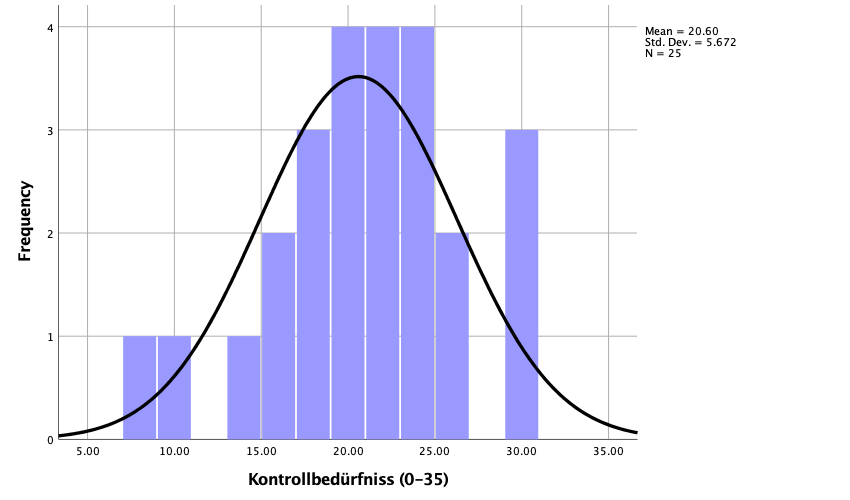
\includegraphics[width=0.85\textwidth]{graphics/histogramm_need-for-control.png}
			\caption{
				\label{fig:histogramm_need-for-control.png} 
				Histogramm des Kontrollbedürfnisses der Probenden. (0 - kein Kontrollbedürfnis, 35 - volles Kontrollbedürfnis)
			}
		\end{figure}
	\end{frame}

%%% FEATURES %%%

\begin{comment}

	\begin{frame}[fragile]{Typography}
		\begin{verbatim}The theme provides sensible defaults to
		\emph{emphasize} text, \alert{accent} parts
		or show \textbf{bold} results.\end{verbatim}

		\begin{center}becomes\end{center}

		The theme provides sensible defaults to \emph{emphasize} text,
		\alert{accent} parts or show \textbf{bold} results.
	\end{frame}

	\begin{frame}{Font feature test}
		\begin{itemize}
			\item Regular
			\item \textit{Italic}
			\item \textsc{Small Caps}
			\item \textbf{Bold}
			\item \textbf{\textit{Bold Italic}}
			\item \textbf{\textsc{Bold Small Caps}}
			\item \texttt{Monospace}
			\item \texttt{\textit{Monospace Italic}}
			\item \texttt{\textbf{Monospace Bold}}
			\item \texttt{\textbf{\textit{Monospace Bold Italic}}}
		\end{itemize}
	\end{frame}

	\begin{frame}{Lists}
		\begin{columns}[T,onlytextwidth]
			
			\column{0.33\textwidth}
			Items
			\begin{itemize}
				\item Milk \item Eggs \item Potatoes
			\end{itemize}

			\column{0.33\textwidth}
			Enumerations
			\begin{enumerate}
				\item First, \item Second and \item Last.
			\end{enumerate}

			\column{0.33\textwidth}
			Descriptions
			\begin{description}
				\item[PowerPoint] Meeh. \item[Beamer] Yeeeha.
			\end{description}
		\end{columns}
	\end{frame}

	\begin{frame}{Animation}
		\begin{itemize}[<+- | alert@+>]
			\item \alert<4>{This is\only<4>{ really} important}
			\item Now this
			\item And now this
		\end{itemize}
	\end{frame}

	\begin{frame}{Tables}
		\begin{table}
			\caption{Largest cities in the world (source: Wikipedia)}
			\begin{tabular}{@{} lr @{}}
				\toprule
				City & Population\\
				\midrule
				Mexico City & 20,116,842\\
				Shanghai & 19,210,000\\
				Peking & 15,796,450\\
				Istanbul & 14,160,467\\
				\bottomrule
			\end{tabular}
		\end{table}
	\end{frame}

	\begin{frame}{Blocks}
		Three different block environments are pre-defined and may be styled with an
		optional background color.

		\begin{columns}[T,onlytextwidth]
			
			\column{0.5\textwidth}
			\begin{block}{Default}
				Block content.
			\end{block}

			\begin{alertblock}{Alert}
				Block content.
			\end{alertblock}

			\begin{exampleblock}{Example}
				Block content.
			\end{exampleblock}

			\column{0.5\textwidth}
			\metroset{block=fill}
			\begin{block}{Default}
				Block content.
			\end{block}

			\begin{alertblock}{Alert}
				Block content.
			\end{alertblock}

			\begin{exampleblock}{Example}
				Block content.
			\end{exampleblock}

		\end{columns}
	\end{frame}

	\begin{frame}{Quotes}
		\begin{quote}
			Veni, Vidi, Vici
		\end{quote}
	\end{frame}

	\begin{frame}{References}
		Some references to showcase [allowframebreaks] \cite{knuth92,ConcreteMath,Er01,greenwade93}
	\end{frame}

\end{comment}

\end{document}